\documentclass[letterpaper,12pt]{article}
\usepackage{enumitem}
\usepackage[utf8]{inputenc}
\usepackage{amsmath}
\usepackage[T1]{fontenc}
\usepackage[polish]{babel}
\usepackage{geometry}
\geometry{margin=2.5cm}
\usepackage{lmodern}
\usepackage{dirtytalk}
\usepackage{graphicx}
\usepackage{mathtools}
\usepackage{enumitem}
\usepackage{mathrsfs}
\usepackage{float}
\let\lll\relax
\usepackage{amssymb}
\usepackage{bbm}
\usepackage{amsthm}
\usepackage{hyperref}
\usepackage{cleveref}
\usepackage{indentfirst}
\usepackage{microtype}
\binoppenalty=10000
\relpenalty=10000
\setlength{\emergencystretch}{3em}
\newtheorem{definition}{Definicja}
\newtheorem{fact}{Fakt}
\newtheorem{conclusion}{Wniosek}
\newtheorem{lemma}{Lemat}
\crefname{lemma}{Lemat}{Lematy}
\newtheorem{theorem}{Twierdzenie}
\newtheorem{hypothesis}{Hipoteza}
\addto\captionspolish{
  \renewcommand\tablename{Tabela}
  }
\usepackage{listings}
\usepackage{xcolor}
\usepackage[numbers]{natbib}
\allowdisplaybreaks

\begin{document}
\begin{titlepage}
  \centering
  {\Large\bfseries Politechnika Wrocławska \par}

  {\large\bfseries Wydział Informatyki i Telekomunikacji \par}
  \rule{\textwidth}{0.2pt}\\[1cm]

  {\raggedright
  {\small Kierunek:}
  {\small\bfseries Informatyka algorytmiczna (INA)}\\[3cm]}

  {\Huge\bfseries PRACA DYPLOMOWA\\[4mm] INŻYNIERSKA}\\[3cm]

  {\huge\bfseries Modularity i jego modyfikacje w rodzinach grafów gęstych}\\[1.5cm]

  {\LARGE\bfseries Zofia Kuriata}\\[2cm]

  {\Large Opiekun pracy}\\[3mm]
  {\Large\bfseries dr inż. Małgorzata Sulkowska}\\[2.5cm]

  {\raggedright
  {\large Słowa kluczowe: modularity, społeczność, grafy gęste}\\[3mm]
  \rule{\textwidth}{0.6pt}\\}

  {\large WROCŁAW 2025}
\end{titlepage}

\newpage
\section*{Streszczenie}
Modularity jest miarą jakości podziału grafu na społeczności. Posiada wiele zastosowań w analizie sieci społecznych, biologicznych czy informatycznych. W literaturze większość badań dotyczy grafów rzadkich, w tej pracy natomiast skupimy się na grafach gęstych. Skoncentrujemy się na badaniu modularity oraz jego zmodyfikowanej wersji - modularity star. Modularity star eliminuje niektóre wady klasycznej wersji modularity, zwracając bardziej intuicyjne wartości.\\
\indent Celem pracy jest sprawdzenie, które własności modularity można przenieść na modularity star oraz zbadanie różnic między tymi dwoma miarami w kontekście rodzin grafów gęstych. Zaproponujemy ograniczenie górne na modularity star oraz odpowiemy na pytanie o minimalną liczbę krawędzi, które należy usunąć z grafów gęstych, aby ich modularity star stało się dodatnie. Zadamy również pytanie: czy istnieje graf, dla którego modularity star jest większe niż modularity oraz przedstawimy hipotetyczną odpowiedź.

\section*{Abstract}
Modularity is a widely used measure for evaluating the quality of a graph partition into communities. It plays an important role in the analysis of social, biological, and information networks. While most existing research focuses on sparse graphs, this work examines the behavior of modularity in the setting of dense graphs. In particular, we study both the classical modularity measure and its modification, modularity star. The modified version eliminates some drawbacks of the classical version of modularity, returning more intuitive values.\\
\indent The objective of this thesis is to determine which known properties of modularity carry over to modularity star and to investigate the differences between these two measures in the context of dense graph families. We establish an upper bound for modularity star and determine the minimal number of edges that must be removed from dense graphs in order for their modularity star value to become positive. We also consider the open question of whether there exists a graph for which modularity star exceeds classical modularity, and we discuss arguments suggesting that this may indeed be the case.

\newpage
\tableofcontents
\newpage

\section*{Wprowadzenie}
\addcontentsline{toc}{section}{\protect\numberline{}Wprowadzenie}
Wiele sieci rzeczywistych - społecznych, biologicznych czy informatycznych - wykazuje strukturę społecznościową, w której węzły tworzą grupy o gęstszych powiązaniach wewnętrznych niż zewnętrznych. Jako miarę jakości podziału grafu na społeczności często wykorzystuje się \textit{modularity}. Parametr ten został zaproponowany przez Newmana i Girvana w 2004 roku~\cite{NG04}. Tzw. modularity score mierzy jakość struktury społecznościowej danego podziału grafu, porównując liczbę krawędzi wewnętrznych w społecznościach z oczekiwaną liczbą krawędzi w losowym grafie o takim samym rozkładzie stopni wierzchołków. Popularne algorytmy klasteryzacji, takie jak algorytmy Louvain oraz Leiden, próbują optymalizować modularity score w celu wykrywania społeczności w sieciach \cite{BGLL08, TWE19}.\\
\indent Jednak modularity posiada pewne wady. Na przykład, wykazuje tzw. \textit{resolution limit}, co oznacza, że może nie wykrywać małych społeczności w dużych sieciach \cite{FB07, K24}. Ponadto, może przyjmować wysokie wartości dla niektórych rodzin grafów, które nie posiadają wyraźnej struktury społecznościowej. Przykłady takich rodzin to kraty \cite{K24}, drzewa o maksymalnym stopniu podliniowym z liczbą wierzchołków \cite{MS18} oraz grafy z wykluczonym minorem o maksymalnym stopniu podliniowym z liczbą wierzchołków \cite{LS23}. Jedna z modyfikacji modularity - \textit{modularity star}, eliminuje niektóre z wad klasycznej wersji, zwracając bardziej intuicyjne wartości dla konkretnych rodzin grafów.\\
\indent W literaturze jest niewiele badań dotyczących grafów gęstych. Większość prac koncentruje się na grafach rzadkich, które odpowiadają sieciom rzeczywistym. Postaramy się częściowo wypełnić tę lukę. W pracy tej skupimy się na badaniu modularity oraz modularity star, w kontekście rodzin grafów gęstych. Wyniki dotyczące modularity dla grafów gęstych zawarte są w pracy \cite{MS23}. Naszym celem jest przeniesienie ich na modularity star. W szczególności, przedstawimy ograniczenie górne na modularity star oraz odpowiemy na pytanie o minimalną liczbę krawędzi, które należy usunąć z grafów pełnych oraz pełnych dwudzielnych, aby ich modularity star stało się dodatnie. Poruszymy również pytanie otwarte: czy istnieje graf, dla którego modularity star jest większe niż modularity przedstawiając przesłanki, które pozwalają sądzić, że tak. Nowe, teoretyczne wyniki dla modularity star otrzymane w ramach tej pracy zostały zaprezentowane w twierdzeniach \ref{dinh_thai_star}, \ref{f_star}, \ref{delta_star}.\\
\indent Praca ma na celu pogłębienie zrozumienia modularity star w kontekście grafów gęstych oraz dostarczenie nowych narzędzi i wyników, które mogą być użyteczne w dalszych badaniach nad wykrywaniem społeczności w sieciach.
\newpage

\section{Definicje}
Rozdział ten przedstawia notację oraz potrzebne w dalszej części pracy definicje grafowe.
\subsection{Podstawowe definicje grafowe}
\begin{definition}
  (\textbf{Graf}) Graf \(G\) prosty nieskierowany to para \((V, E)\), gdzie
  \begin{itemize}
    \item \(V\) - skończony zbiór wierzchołków,
    \item \(E \subseteq \{\{u,v\}: u,v \in V, u \neq v\}\). Krawędź \(e\) jest incydentna z wierzchołkiem \(v\), jeśli \(v \in e\).
  \end{itemize}
\end{definition}
Za graf będziemy uważać graf prosty nieskierowany. Para \((V, E)\) będzie domyślnie utożsamiana z \(G\).\\

\begin{definition}
  (\textbf{Graf pełny}) Graf pełny to \(K_n = (V,E)\), gdzie
  \begin{itemize}
    \item \(V = \{v_1, \ldots, v_n\}\),
    \item \(E = \{\{v_i, v_j\} : 1 \leq i < j \leq n\}\).
  \end{itemize}
\end{definition}
Zatem graf pełny to graf, w którym każdy wierzchołek jest połączony z każdym innym dokładnie jedną krawędzią.\\

\begin{definition}
  (\textbf{Graf pełny dwudzielny}) Graf pełny dwudzielny to \(K_{s,t} = (S \cup T,E)\), gdzie
  \begin{itemize}
    \item \(|S|=s\), \(|T|=t\) oraz \(S\), \(T\) - zbiory rozłączne,
    \item \(E = \{\{v_i, v_j\} : v_i \in S, v_j \in T\}\).\\
  \end{itemize}
\end{definition}

\begin{definition}
  (\textbf{Gwiazda / Star}) Gwiazda \(S_n\) to graf będący szczególnym przypadkiem grafu pełnego dwudzielnego - \(K_{1,n}\).\\
\end{definition}

\begin{definition}
  (\textbf{Ścieżka / Path}) Ścieżka \(P_n=(V,E)\) to graf, taki że \(V=\{v_1, \ldots, v_n\}\), \(E=\{\{v_i, v_{i+1}\}\}\) dla \(1 \leq i < n\).\\
\end{definition}

\begin{definition}
  (\textbf{Stopień wierzchołka w grafie}) Stopień wierzchołka \(v\) w grafie \(G\), oznaczany jako \(deg_G(v)\), to liczba krawędzi incydentnych z wierzchołkiem \(v\):
  \[deg_G(v) = |\{e \in E : v \in e\}|.\]\\
\end{definition}

\begin{definition}
  (\textbf{Partycja zbioru wierzchołków}) Niech \(G = (V, E)\) będzie grafem. Partycja zbioru wierzchołków \(V\) to zbiór \(\mathcal{A} = \{A_1, A_2, \ldots, A_k\}\), gdzie
  \begin{itemize}
    \item \(\forall_{i=1}^k A_i \subseteq V\),
    \item \(\forall_{1 \leq i < j \leq k} A_i \cap A_j = \emptyset\),
    \item \(\bigcup_{i=1}^{k} A_i = V\).
  \end{itemize}
  Element partycji \(A_i\) będziemy nazywać \textbf{społecznością}.\\
\end{definition}

\begin{definition}
  (\textbf{Podgraf indukowany}) Niech \(G = (V, E)\) będzie grafem, \(W \subseteq V\). Graf \(H = (W, F)\) nazywamy podgrafem \(G\) indukowanym przez \(W\), jeśli \(F = W^{[2]} \cap E\), gdzie \(W^{[2]}\) to zbiór wszystkich dwuelementowych podzbiorów zbioru \(W\). Oznaczamy jako \(H=G[W]\).\\
\end{definition}

\subsection{Oznaczenia}
Niech \(G = (V, E)\) będzie grafem oraz \(A, B \subseteq V\), wtedy
\begin{itemize}
  \item \(A^c = V \setminus A\),
  \item \(e(A) = |\{ \{u, v\} \in E : u \in A, v \in A\}|\) - liczba krawędzi wewnętrznych w społeczności \(A\) w grafie \(G=(V,E)\), jeśli konieczne będzie wskazanie grafu, to będziemy oznaczać jako \(e_G(A)\),
  \item \(e(A, B) = |\{ \{u, v\} \in E : u \in A, v \in B\}|\) - liczba krawędzi pomiędzy społecznościami \(A\) oraz \(B\) w grafie \(G=(V,E)\), jeśli konieczne będzie wskazanie grafu, to będziemy oznaczać jako \(e_G(A, B)\),
  \item \(e(G) = |E|\) - liczba krawędzi w grafie \(G\),
  \item \(vol(A) = \sum_{u \in A}deg_G(u)\) - suma stopni wierzchołków w danym podzbiorze wierzchołków \(A\), jeśli konieczne będzie wskazanie grafu, to będziemy oznaczać jako \(vol_G(A)\),
  \item \(vol(G) = 2e(G)\) - suma stopni wszystkich wierzchołków w grafie \(G\),
  \item \(p_G(A) = 2e(A) \cdot vol(G) - {vol(A)}^2,\)
  \item \(\delta^{-}(G)\) - minimalna liczba krawędzi, które należy usunąć z grafu \(G\), aby \(mod(G') > 0\),
  \item \(\delta^{-}_*(G)\) - minimalna liczba krawędzi, które należy usunąć z grafu \(G\), aby \(mod^*(G') > 0\).
\end{itemize}

\section{Modularity}
Modularity jest jedną z miar jakości podziału grafu na społeczności. Nie uwzględnia ona wewnętrznych struktur społeczności, a jedynie liczbę ich wewnętrznych krawędzi oraz sumę stopni ich wierzchołków. Modularity osiąga wysokie watości, jeżeli dla danego grafu istnieje partycjonowanie zbioru jego wierzchołków na podzbiory, takie że liczba ich krawędzi wewnętrznych jest większa niż oczekiwana w losowym grafie o takim samym ciągu stopni wierzchołków.\\
W ogólności, problem wyznaczenia modularity grafu jest NP-zupełny \cite[Section 4]{BD08}.
W celu wyznaczenia modularity grafu, należy rozpatrzyć wszystkie możliwe partycje zbioru wierzchołków grafu \(G\) i wybrać tę, której wartość tzw. \textit{modularity score} jest największa.\\

\subsection{Definicja modularity} \label{def_mod}
\begin{definition}
  (\textbf{Modularity społeczności}) Niech \(G = (V, E)\) będzie grafem z co najmniej jedną krawędzią, \(A \subseteq V\). Wtedy \textbf{modularity społeczności} \(A\) w grafie \(G\) definiujemy jako
  \[
    mod_A(G) = \frac{e(A)}{e(G)} - {\left(\frac{vol(A)}{vol(G)}\right)}^2.
  \]
\end{definition}
Pierwszy składnik \(\frac{e(A)}{e(G)}\) będziemy oznaczać jako \textbf{\(EC_G(A)\) - edge contribution}, a drugi \({\left(\frac{vol(A)}{vol(G)}\right)}^2\) jako \textbf{\(DT_G(A)\) -  degree tax}.\\

Widzimy zatem, że w kontekście modularity, udział krawędzi w danym podzbiorze jest promowany, podczas gdy udział stopni wierzchołków jest karany.\\

\begin{definition}
  (\textbf{Modularity score}) Niech \(G = (V, E)\) będzie grafem z co najmniej jedną krawędzią, \(\mathcal{A}\) będzie partycją zbioru wierzchołków \(G\). Wtedy \textbf{modularity score} partycji \(\mathcal{A}\) w grafie \(G\) definiujemy jako
  \[
    mod_{\mathcal{A}}(G) = \sum_{A \in \mathcal{A}} \left(\frac{e(A)}{e(G)} - {\left(\frac{vol(A)}{vol(G)}\right)}^2\right) = \sum_{A \in \mathcal{A}} mod_A(G).
  \]
\end{definition}
Jako \textbf{\(EC_{\mathcal{A}}(G)\)} będziemy oznaczać sumę wszystkich \(EC_G(A)\) dla \(A \in \mathcal{A}\), a jako \textbf{\(DT_{\mathcal{A}}(G)\)} sumę wszystkich \(DT_G(A)\) dla \(A \in \mathcal{A}\).\\

\begin{definition}
  (\textbf{Modularity grafu}) Niech \(G = (V, E)\) będzie grafem z co najmniej jedną krawędzią. Wtedy \textbf{modularity grafu} \(G\) definiujemy jako
  \[
    mod(G) = \max_{\mathcal{A} \in \mathcal{P}(V)} mod_{\mathcal{A}}(G),
  \]
  gdzie \(\mathcal{P}(V)\) to zbiór wszystkich partycji zbioru wierzchołków grafu \(G\).\\

  Dla grafu bez krawędzi przyjmujemy wartość \textbf{modularity} równą \textbf{0}.
\end{definition}

Poniżej przedstawione zostały trzy alternatywne postacie \textbf{modularity score}.
\begin{lemma}
  Niech \(G = (V, E)\) będzie grafem z co najmniej jedną krawędzią, \(\mathcal{A}\) będzie partycją zbioru wierzchołków \(G\). Wtedy \textbf{modularity score} partycji \(\mathcal{A}\) w grafie \(G\) spełnia
  \[mod_{\mathcal{A}}(G) = \sum_{A \in \mathcal{A}} \frac{p_G(A)}{vol(G)^2}.\]
\end{lemma}

\begin{proof}
  Mamy
  \begin{align*}
    \sum_{A \in \mathcal{A}} \frac{p_G(A)}{vol(G)^2} & = \sum_{A \in \mathcal{A}} \frac{2e(A) \cdot vol(G) - {vol(A)}^2}{vol(G)^2}                           \\
                                                     & = \sum_{A \in \mathcal{A}} \left(\frac{2e(A)}{vol(G)} - {\left(\frac{vol(A)}{vol(G)}\right)}^2\right) \\
                                                     & = \sum_{A \in \mathcal{A}} \left(\frac{e(A)}{e(G)} - {\left(\frac{vol(A)}{vol(G)}\right)}^2\right)    \\
                                                     & = mod_{\mathcal{A}}(G).
  \end{align*}
\end{proof}

\begin{lemma}
  \label{score_deg}
  Niech \(G = (V, E)\) będzie grafem z co najmniej jedną krawędzią, \(\mathcal{A}\) będzie partycją zbioru wierzchołków \(G\). Wtedy \textbf{modularity score} partycji \(\mathcal{A}\) w grafie \(G\) spełnia
  \[mod_{\mathcal{A}}(G) = \frac{1}{vol(G)}\sum_{A \in \mathcal{A}} \sum_{u,v \in A} \left( \mathbbm{1}_{\{u,v\} \in E} - \frac{deg_G(u) \cdot deg_G(v)}{vol(G)}\right).\]
\end{lemma}

\begin{proof}
  Mamy
  \begin{align*}
     & \frac{1}{vol(G)}\sum_{A \in \mathcal{A}} \sum_{u,v \in A}
    \left( \mathbbm{1}_{\{u,v\} \in E} - \frac{deg_G(u) \cdot deg_G(v)}{vol(G)}\right) \\
     & = \frac{1}{vol(G)}\sum_{A \in \mathcal{A}}
    \left( 2e(A) - \frac{1}{vol(G)} \sum_{u,v \in A} deg_G(u) \cdot deg_G(v)\right)    \\
     & = \frac{1}{vol(G)}\sum_{A \in \mathcal{A}}
    \left( 2e(A) - \frac{vol(A)^2}{vol(G)}\right)                                      \\
     & = \sum_{A \in \mathcal{A}}
    \left(\frac{e(A)}{e(G)} - {\left(\frac{vol(A)}{vol(G)}\right)}^2\right) = mod_{\mathcal{A}}(G).
  \end{align*}
\end{proof}

\begin{lemma}
  \label{2partition}
  Niech \(G = (V, E)\) będzie grafem z co najmniej jedną krawędzią, \(\mathcal{A}=\{A_1,A_2\}\) będzie dwuelementową partycją zbioru wierzchołków \(G\). Wtedy \textbf{modularity score} partycji \(\mathcal{A}\) w grafie \(G\) spełnia
  \[mod_{\mathcal{A}}(G) = \frac{8e(A_1)e(A_2)-2e(A_1,A_2)^2}{vol(G)^2}.\]
\end{lemma}

\begin{proof}
  Zauważmy, że
  \begin{align*}
    mod_{A_1}(G) & = \frac{e(A_1)}{e(G)} - \left(\frac{vol(A_1)}{vol(G)}\right)^2                    \\
                 & = \frac{e(A_1)\cdot 4e(G) - vol(A_1)^2}{vol(G)^2}                                 \\
                 & = \frac{e(A_1)\cdot 4e(G) - (2e(A_1)+e(A_1, A_2))^2}{vol(G)^2}                    \\
                 & = \frac{e(A_1)\cdot 4e(G) - 4e(A_1)^2-4e(A_1)e(A_1, A_2)-e(A_1, A_2)^2}{vol(G)^2} \\
                 & = \frac{4e(A_1)(e(G)-e(A_1)-e(A_1, A_2))-e(A_1, A_2)^2}{vol(G)^2}                 \\
                 & = \frac{4e(A_1)e(A_2)-e(A_1, A_2)^2}{vol(G)^2}.
  \end{align*}
  Symetrycznie
  \[mod_{A_2}(G) = \frac{4e(A_2)e(A_1)-e(A_2, A_1)^2}{vol(G)^2}.\]
  A zatem
  \begin{align*}
    mod_{\mathcal{A}}(G) & = mod_{A_1}(G) + mod_{A_2}(G)                     \\
                         & = \frac{8e(A_1)e(A_2) - 2e(A_1,A_2)^2}{vol(G)^2}.
  \end{align*}
\end{proof}

\subsection{Podstawowe własności modularity} \label{własności}
\begin{fact} \cite[Lemma 3.1]{BD08}
  \label{score_bounds}
  Niech \(G = (V,E)\) będzie grafem z co najmniej jedną krawędzią, \(\mathcal{A}\) partycją wierzchołków \(G\). Wtedy
  \[-\frac{1}{2} \leq mod_{\mathcal{A}}(G) < 1.\]
\end{fact}
\begin{proof}
  Niech \(G = (V,E)\) będzie grafem z co najmniej jedną krawędzią, \(\mathcal{A}\) k-elementową partycją zbioru wierzchołków \(G\).\\

  Zaczniemy od ograniczenia dolnego. Wkład każdej społeczności \(A \in \mathcal{A}\) modularity score wynosi
  \begin{align*}
    mod_A(G) & = \frac{e(A)}{e(G)} - {\left(\frac{vol(A)}{vol(G)}\right)}^2          \\
             & = \frac{e(A)}{e(G)} - {\left(\frac{2e(A)+e(A,A^c)}{vol(G)}\right)}^2. \\
    % &= \frac{4e(A)e(G)-4e(A)^2-4e(A)e(A, A^c)-e(A, A^c)}{4e(G)^2}
  \end{align*}
  Powyższe wyrażenie maleje wraz ze wzrostem \(e(A, A^c)\) oraz osiąga minimum względem \(e(A)\) dla \(e(A) = 0\). Zatem minimalna wartość \(mod_A(G)\) jest osiągana, gdy \(e(A) = 0\) oraz \(e(A, A^c)\) jest maksymalne. Wiedząc, że \((a+b)^2 \geq a^2+b^2\), dla \(a,b \geq 0\), możemy stwierdzić, że modularity score partycji \(\mathcal{A}\) osiąga minimum, gdy zawiera ona dokładnie dwie społeczności oraz wszystkie krawędzie grafu \(G\) leżą pomiędzy tymi społecznościami.\\

  Niech \(\mathcal{A}=\{A_1,A_2\}\). Wtedy
  \[mod_{\mathcal{A}}(G) = -\frac{vol(A_1)^2+vol(A_2)^2}{(vol(A_1)+vol(A_2))^2}.\]
  Zauważmy, że jeśli jedyne krawędzie w grafie leżą pomiędzy społecznościami \(A_1\) oraz \(A_2\), to \(vol(A_1)=vol(A_2)\). Wtedy
  \[mod_{\mathcal{A}}(G) = \frac{vol(A_1)^2+vol(A_1)^2}{(vol(A_1)+vol(A_1))^2} = -\frac{1}{2}.\]\\
  Przykładem grafu i partycji zbioru jego wierzchołków realizującej to minimum jest graf dwudzielny z partycją, w której każda z dwóch społeczności odpowiada jednej części grafu dwudzielnego, która nie posiada krawędzi wewnętrznych. Został on przedstawiony na rysunku \ref{minimum_mod}.\\

  \begin{figure}[H]
    \centering
    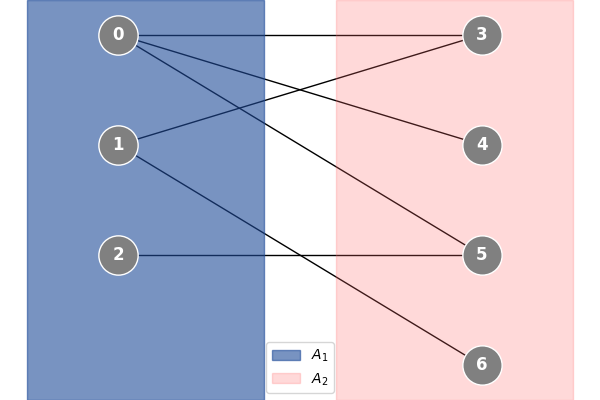
\includegraphics[width=0.7\textwidth]{../graphs/minimum_mod.png}
    \caption{Partycja zbioru wierzchołków grafu dwudzielnego realizująca minimalną wartość modularity score.}
    \label{minimum_mod}
  \end{figure}

  Przejdźmy do ograniczenia górnego. \(EC_{\mathcal{A}}(G)\) jest na pewno nie większa niż 1. Ale z założenia, graf ma co najmniej jedną krawędź, więc suma \(DT_{\mathcal{A}}(G)\) w dowolnym partycjonowaniu jest dodatnia. Zatem modularity nie może osiągnąć wartości 1, czyli
  \[mod_{\mathcal{A}}(G) < 1.\]
\end{proof}

\begin{fact}
  Niech \(G = (V,E)\) będzie grafem z co najmniej jedną krawędzią, wtedy \(mod(G) \geq 0\).
\end{fact}
\begin{proof}
  Wartość modularity score dla partycjonowania \(\mathcal{A}\), w którym wszystkie wierzchołki grafu \(G\) należą do jednej społeczności, jest równa 0 (\(EC_{\mathcal{A}}(G) = DT_{\mathcal{A}}(G) = 1\)). Takie partycjonowanie możemy osiągnąć dla dowolnego grafu.
\end{proof}

\begin{conclusion}
  Niech \(G = (V,E)\) będzie grafem z co najmniej jedną krawędzią, wtedy
  \[0 \leq mod(G) < 1.\]
\end{conclusion}

\begin{fact}
  Izolowane wierzchołki nie mają wpływu na modularity grafu.
\end{fact}
Wierzchołki stopnia zerowego nie mają wkładu ani do \textit{edge contribution}, ani do \textit{degree tax}. Zatem nie mają wpływu na modularity grafu.\\

Od tej pory, w kontekście modularity, będziemy ignorować izolowane wierzchołki i założymy, że rozważane przez nas grafy ich nie posiadają.\\

\begin{lemma}\cite[Lemma 2]{DXT09}
  Niech \(G = (V,E)\) będzie grafem z co najmniej jedną krawędzią, \(\mathcal{A}\) partycją, dla której \(mod_{\mathcal{A}}(G) = mod(G)\). Wtedy każda społeczność w partycji \(\mathcal{A}\) kontrybuuje nieujemnie do wartości modularity grafu \(G\), tzn.
  \[\forall_{A \in \mathcal{A}} \hspace{1mm} mod_A(G) \geq 0 .\]
\end{lemma}

\begin{proof}
  Załóżmy niewprost, że istnieje partycja zbioru wierzchołków \(G\) \(\mathcal{A} = \{A_1, A_2, \ldots, A_s, B\}\), \(mod_B(G) < 0\) oraz że połączenie \(B\) z jakąkolwiek inną społecznością w \(\mathcal{A}\) nie zwiększy wartości \(mod_{\mathcal{A}}(G)\). Wiemy, że
  \[mod_B(G) = \frac{e(B)}{e(G)} - {\left(\frac{vol(B)}{vol(G)}\right)}^2 < 0,\]
  \[\forall_{1 \leq i \leq s} \hspace{1mm} mod_{A_i}(G) = \frac{e(A_i)}{e(G)} - {\left(\frac{vol(A_i)}{vol(G)}\right)}^2,\]
  \[\forall_{1 \leq i \leq s} \hspace{1mm} mod_{B \cup A_i}(G) = \frac{e(A_i)+e(B)+e(A_i, B)}{e(G)} - {\left(\frac{vol(A_i)+vol(B)}{vol(G)}\right)}^2.\]
  Zatem
  \[\forall_{1 \leq i \leq s} \hspace{1mm} mod_{B \cup A_i}(G)-mod_B(G)-mod_{A_i}(G) = \frac{e(A_i, B)}{e(G)} - \frac{2vol(A_i)vol(B)}{vol(G)^2} \leq 0.\]
  Zsumujmy te nierówności dla \(i=1, 2, \ldots, s\)
  \begin{align*}
     & \sum_{i=1}^{s} \left(\frac{e(A_i, B)}{e(G)} - \frac{2vol(A_i)vol(B)}{vol(G)^2} \right) \leq 0 \\
     & \frac{e(B, B^c)}{e(G)} - \frac{2vol(B)}{vol(G)^2} \cdot (vol(G)-vol(B)) \leq 0                \\
     & \frac{vol(B)-2e(B)}{e(G)} + \frac{2vol(B)^2}{vol(G)^2} - \frac{2vol(B)}{vol(G)} \leq 0        \\
     & -2mod_B(G) + \frac{vol(B)}{e(G)} - \frac{2vol(B)}{2e(G)} \leq 0                               \\
     & -2mod_B(G) \leq 0                                                                             \\
     & mod_B(G) \geq 0.
  \end{align*}
  Otrzymujemy sprzeczność, ponieważ założyliśmy, że \(mod_B(G) < 0\).\\
  Zatem jeśli w dowolnej partycji istnieje społeczność o ujemnym wkładzie do modularity score, to możemy znaleźć takie połączenie jej z inną społecznością, które zwiększa wartość modularity score nowo powstałej partycji.\\
  Czyli optymalne partycjonowanie nie może zawierać społeczności o ujemnym wkładzie do modularity grafu \(G\).\\
\end{proof}

\begin{fact}
  Niech \(G = (V,E)\) będzie grafem, \(\mathcal{A}\) partycją, dla której \(mod_{\mathcal{A}}(G) = mod(G)\). Wtedy każda społeczność w partycji \(\mathcal{A}\) indukuje podgraf spójny.
\end{fact}

\begin{proof}
  Załóżmy niewprost, że istnieje społeczność \(A\) indukująca niespójny podgraf w partycji \(\mathcal{A}\). Niech \(A_1\) i \(A_2\) będą podzbiorami \(A\), takimi że \(A = A_1 \cup A_2\) oraz \(e(A) = e(A_1) + e(A_2)\). Wtedy \(vol(A) = vol(A_1) + vol(A_2)\) oraz
  \[ mod_A(G) = \frac{e(A)}{e(G)} - {\left(\frac{vol(A)}{vol(G)}\right)}^2,\]
  \[ mod_{A_1}(G) + mod_{A_2}(G) = \frac{e(A_1)+e(A_2)}{e(G)} - {\left(\frac{vol(A_1)}{vol(G)}\right)}^2 - {\left(\frac{vol(A_2)}{vol(G)}\right)}^2.\]

  Zatem
  \begin{align*}
    mod_{A_1}(G) + mod_{A_2}(G) - mod_A(G)
     & = \frac{{vol(A)}^2 - {vol(A_1)}^2 - {vol(A_2)}^2}{4e(G)^2} \\
     & = \frac{2vol(A_1)vol(A_2)}{4e(G)^2} > 0.
  \end{align*}

  Czyli partycjonowanie zapewniające maksymalną wartość modularity nie może zawierać społeczności indukującej niespójne podgrafy.\\
\end{proof}

\begin{fact}
  Niech \(G = (V,E)\) będzie grafem z co najmniej jedną krawędzią, \(\mathcal{A}\) partycją, dla której \(mod_{\mathcal{A}}(G) = mod(G)\). Wtedy partycja \(\mathcal{A}\) nie zawiera społeczności składającej się z pojedynczego wierzchołka stopnia 1.
\end{fact}

\begin{proof}
  Załóżmy niewprost, że w partycji \(\mathcal{A}\) istnieje społeczność \(A\) będąca podgrafem składającym się z pojedynczego wierzchołka (\(v\)) stopnia 1 oraz społeczność \(B\) zawierająca sąsiada \(v\). Wtedy
  \[
    mod_A(G) = \frac{0}{e(G)} - {\left(\frac{1}{vol(G)}\right)}^2 = -\frac{1}{vol(G)^2},
  \]
  \[
    mod_B(G) = \frac{e(B)}{e(G)} - {\left(\frac{vol(B)}{vol(G)}\right)}^2.
  \]
  Natomiast
  \[
    mod_{A \cup B}(G) = \frac{e(B)+1}{e(G)} - {\left(\frac{vol(B)+1}{vol(G)}\right)}^2.
  \]
  Zatem
  \begin{align*}
    mod_{A \cup B}(G) - \left(mod_A(G)+mod_B(G)\right)
     & = \frac{1}{e(G)} - \frac{2vol(B)}{vol(G)^2} \\
     & = \frac{vol(G)-vol(B)}{2e(G)^2} > 0.
  \end{align*}
\end{proof}

\subsection{Górne ograniczenie na modularity}
\begin{theorem}
  \label{dinh_thai}
  \cite[Lemma 1]{DT11}
  Niech \(G = (V,E)\) będzie grafem z co najmniej jedną krawędzią, niech \(k \geq 2\). Wtedy
  \[mod(G) \leq \frac{k}{k-1} \cdot \max_{\mathcal{A} : |\mathcal{A}| \leq k} mod_{\mathcal{A}}(G).\]
\end{theorem}

\begin{proof}
  Niech \(\mathcal{A} = \{A_1, A_2, \ldots, A_t\}\) będzie partycją zbioru wierzchołków \(G\), dla której \(mod_{\mathcal{A}}(G) = mod(G)\).\\
  Jeśli \(t \leq k\), to teza jest oczywiście spełniona. Załóżmy zatem, że \(t > k\).\\
  Stworzymy partycję \(\mathcal{B}\) poprzez pogrupowanie społeczności z \(\mathcal{A}\) w \(l \leq k\) zbiorów \(B_1, B_2, \ldots, B_l\).\\
  Zrobimy to następująco: dla każdej społeczności \(A_i \in \mathcal{A}\) wybieramy jednostajnie losowo i niezależnie liczbę \(j \in \{1, 2, \ldots, k\}\) i dodajemy \(A_i\) do zbioru \(B_j\). Otrzymane niepuste zbiory tworzą partycję \(\mathcal{B}\).\\

  Z lematu \ref{score_deg} wiemy, że modularity score partycji \(\mathcal{A}\) jest równe
  \[
    mod_{\mathcal{A}}(G) = \frac{1}{vol(G)} \cdot \sum_{u,v \in V} \left( \mathbbm{1}_{\{u,v\} \in E} - \frac{deg_G(u) \cdot deg_G(v)}{vol(G)}\right) \cdot X_{uv},
  \]
  gdzie
  \[
    X_{uv} = \begin{cases}
      1 & \text{jeśli } u \text{ i } v \text{ należą do tej samej społeczności w } \mathcal{A}, \\
      0 & \text{w przeciwnym razie.}
    \end{cases}
  \]
  Oznaczmy przez \(C_{u,v} = \mathbbm{1}_{\{u,v\} \in E} - \frac{deg_G(u) \cdot deg_G(v)}{vol(G)}\).\\
  W celu uproszczenia zapisu poprzez \(\sum_{X_{uv} = 0} C_{u,v}\) będziemy rozumieć \(\sum_{\substack{u,v \in V \\\land X_{uv} = 0}} C_{u,v}\). Analogicznie poprzez \(\sum_{X_{uv} = 1} C_{u,v}\) będziemy rozumieć \(\sum_{\substack{u,v \in V \\\land X_{uv} = 1}} C_{u,v}\).

  Teraz modularity score partycji \(\mathcal{A}\) możemy zapisać jako
  \[
    mod_{\mathcal{A}}(G) = \frac{1}{vol(G)} \cdot \sum_{X_{uv} = 1} C_{u,v}.
  \]

  Zastanówmy się nad wartością oczekiwaną \(mod_{\mathcal{B}}(G)\).
  \begin{itemize}
    \item Jeśli \(X_{uv} = 1\), to \(u\) i \(v\) należą do tej samej społeczności w \(\mathcal{A}\), więc należą do tej samej społeczności również w \(\mathcal{B}\) - wkład \(C_{u,v}\) zostanie policzony,
    \item Jeśli \(X_{uv} = 0\), to \(u\) i \(v\) należą do różnych społeczności w \(\mathcal{A}\), a z prawdopodobieństwem \(\frac{1}{k}\) trafią do tej samej społeczności w \(\mathcal{B}\) - wkład \(C_{u,v}\) zostanie pomnożony przez \(\frac{1}{k}\).
  \end{itemize}
  Zauważmy, że \(\sum_{u,v \in V} C_{u,v} = 0\), ponieważ dla partycji jednoelementowej \(\mathcal{T}\)\\\(mod_{\mathcal{T}}(G) = \frac{1}{vol(G)} \cdot \sum_{u,v \in V} C_{u,v} = 0\). Zatem
  \[\sum_{X_{uv} = 1} C_{u,v} + \sum_{X_{uv} = 0} C_{u,v} = 0,\]
  \[\sum_{X_{uv} = 0} C_{u,v} = -\sum_{X_{uv} = 1} C_{u,v}.\]

  Wobec tego wartość oczekiwana \(mod_{\mathcal{B}}(G)\) jest równa
  \begin{align*}
    \mathbb{E}[mod_{\mathcal{B}}(G)] & = \frac{1}{vol(G)} \cdot \left(\sum_{X_{uv} = 1} C_{u,v} + \sum_{X_{uv} = 0} C_{u,v} \cdot \frac{1}{k}\right) \\
                                     & = \frac{1}{vol(G)} \cdot \left(\sum_{X_{uv} = 1} C_{u,v} - \sum_{X_{uv} = 1} C_{u,v} \cdot \frac{1}{k}\right) \\
                                     & = \frac{1}{vol(G)} \cdot \left(1-\frac{1}{k}\right) \cdot \sum_{X_{uv} = 1} C_{u,v}                           \\
                                     & = \left(1-\frac{1}{k}\right) \cdot mod_{\mathcal{A}}(G) = \left(1-\frac{1}{k}\right) \cdot mod(G).
  \end{align*}
  A zatem
  \[\max_{\mathcal{B}:|\mathcal{B}|\leq k}mod_{\mathcal{B}}(G) \geq  \left(1-\frac{1}{k}\right) \cdot mod(G),\]
  \[mod(G) \leq \frac{k}{k-1} \cdot \max_{\mathcal{B}:|\mathcal{B}|\leq k}mod_{\mathcal{B}}(G).\]

  Oznacza to, że istnieje partycja zbioru wierzchołków \(V\) o rozmiarze co najwyżej \(k\), której wartość modularity score jest równa co najmniej \(mod(G) \cdot \frac{k-1}{k}\).\\
\end{proof}

Szczególnie interesujący jest dla nas przypadek gdy \(k=2\). Pozwala nam na ograniczenie wartości modularity grafu poprzez przejrzenie jedynie partycji co najwyżej dwuelementowych. Wykorzystamy ten fakt w lemacie poniżej.

\begin{lemma}
  \label{mod_eq}
  Niech \(G = (V,E)\) będzie grafem z co najmniej jedną krawędzią. Wtedy następujące warunki są równoważne
  \begin{enumerate}
    \item \(mod(G) = 0\),
    \item \(mod_{\mathcal{A}}(G) \leq 0\) dla każdej partycji \(\mathcal{A}\) zbioru wierzchołków \(V\), takiej że \(|\mathcal{A}| = 2\),
    \item \(p_G(A) \leq 0\), a zatem również \(mod_A(G) \leq 0\) dla każdego podzbioru \(A \subset V\).
  \end{enumerate}
\end{lemma}

\begin{proof}
  \leavevmode\\
  \indent Zacznijmy od pokazania (2) \(\Leftrightarrow\) (3).\\

  \noindent Niech \(A \subseteq V\) będzie niepustym podzbiorem wierzchołków \(G\), \(A^c = V \setminus A\). Zauważmy, że \(2e(A) = vol(A) - e(A, A^c)\). Mamy
  \begin{align*}
    p_G(A) & = 2e(A) \cdot vol(G) - {vol(A)}^2                                                          \\
           & = \left(vol(A) - e(A, A^c)\right) \cdot vol(G) - vol(A) \cdot \left(vol(G)-vol(A^c)\right) \\
           & = vol(A) \cdot vol(A^c) - e(A, A^c) \cdot vol(G)                                           \\
           & = p_G(A^c).
  \end{align*}
  Niech \(\mathcal{A} = \{A, A^c\}\) będzie partycją \(V\). Wtedy
  \[mod_{\mathcal{A}}(G) = \frac{p_G(A)}{vol(G)^2} + \frac{p_G(A^c)}{vol(G)^2} = \frac{2p_G(A)}{vol(G)^2}.\]

  Zatem jeśli dla każdego niepustego podzbioru \(A \subset V\) zachodzi \(p_G(A) \leq 0\), to dla każdej partycji dwuelementowej \(\mathcal{A}\) zachodzi \(mod_{\mathcal{A}}(G) \leq 0\).\\
  Analogicznie, jeśli nie istnieje partycja dwuelementowa \(\mathcal{A}\), dla której \(mod_{\mathcal{A}}(G) > 0\), to dla każdego niepustego podzbioru \(A \subset V\) zachodzi \(p_G(A) \leq 0\).\\

  Teraz pokażemy (2) \(\Leftrightarrow\) (1).\\

  \noindent Z twierdzenia \ref{dinh_thai} dla \(k=2\) wiemy, że
  \[mod(G) \leq 2 \cdot \max_{\mathcal{A} : |\mathcal{A}| \leq 2} mod_{\mathcal{A}}(G).\]
  Zatem jeśli dla każdej partycji dwuelementowej \(\mathcal{A}\) zachodzi \(mod_{\mathcal{A}}(G) \leq 0\), to modularity grafu \(G\) jest równe 0 (przypomnijmy, że zawsze możemy wybrać partycjonowanie jednoelementowe, dla którego \(mod_{\mathcal{A}}(G) = 0\)).\\

  Jeśli natomiast \(mod(G) = 0\), to oczywiście dla każdej partycji dwuelementowej \(\mathcal{A}\) zachodzi \(mod_{\mathcal{A}}(G) \leq 0\). W przeciwnym razie, gdyby istniała partycja dwuelementowa \(\mathcal{A}\) taka, że \(mod_{\mathcal{A}}(G) > 0\), to modularity grafu \(G\) byłoby większe niż 0.\\

  A zatem warunki (1), (2) i (3) są równoważne.\\
\end{proof}

Powyższy lemat pozwala stwierdzić czy modularity grafu jest równe 0, bez konieczności rozpatrywania wszystkich partycji zbioru wierzchołków - wystarczy przejrzeć jedynie te dwuelementowe.\\

\subsection{Wady modularity} \label{wady}
Klasyczna wersja modularity ma kilka wad i ograniczeń, które powodują otrzymywanie nieintuicyjnych wartości dla pewnych rodzin grafów.
\begin{itemize}
  \item \textbf{Struktura społeczności}. Modularity nie uwzględnia wewnętrznej struktury społeczności. W związku z tym, zarówno społeczność izomorficzna z gwiazdą, jak i społeczność izomorficzna ze ścieżką tego samego rozmiaru i posiadającą tyle samo krawędzi \say{zewnętrznych} w danym grafie, wbrew intuicji, będzie miała tą samą wartość \textit{modularity score}.
  \item \textbf{Resolution limit}. W pewnych przypadkach małe społeczności mogą zostać niewykryte. Weźmy np. graf G, taki że zawiera on dwie, połączone jedną krawędzią, kliki \(K_k\). Okazuje się, że jeśli \(\binom{k}{2} < \frac{\sqrt{2}\sqrt{|E|}-1}{2}\), to w partycjonowaniu \(\mathcal{A}\), dla którego \(mod_{\mathcal{A}}(G)=mod(G)\), obie kliki należą do jednej społeczności. Jest to sprzeczne z naszą intuicją \cite[Twierdzenie 2]{K24}, \cite{FB07}.
  \item \textbf{Nienaturalnie duże wartości}. Modularity przyjmuje bardzo duże wartości dla niektórych klas grafów, które intuicyjnie nie mają wyraźnej struktury społecznościowej. Jak było już wcześniej wspomniane, przykłady takich klas to: klasa krat \cite[Twierdzenie 3]{K24}, klasa drzew o maksymalnym stopniu podliniowym z liczbą wierzchołków \cite{MS18} oraz klasa grafów z wykluczonym minorem o maksymalnym stopniu podliniowym z liczbą wierzchołków \cite{LS23}.
\end{itemize}

\section{Modularity Star}
Jedną z alternatyw dla klasycznej wersji modularity jest \textbf{modularity star}. Modyfikacja polega na przemnożeniu wartości modularity score każdej społeczności w partycji przez \textbf{star factor} - stosunek maksymalnego wewnętrznego stopnia wierzchołka w danej społeczności powiększonego o 1 do liczby wierzchołków w tej społeczności. Obliczenie maksymalnego stopnia nie jest kosztowne obliczeniowo (w przeciwieństwie do obliczania średnicy społeczności). Modularity star promuje społeczności o bardziej zwięzłej strukturze (a zatem te o stosunkowo niewielkiej średnicy), przez co dobrze radzi sobie z problemami opisanymi w rozdziale \ref{wady}.\\

\subsection{Definicja modularity star}
\begin{definition}
  (\textbf{Modularity star score}) Niech \(G = (V, E)\) będzie grafem z co najmniej jedną krawędzią, \(\mathcal{A}\) będzie partycją \(V\). Wtedy \textbf{modularity star score} partycji \(\mathcal{A}\) w grafie \(G\) definiujemy jako
  \[
    mod^*_{\mathcal{A}}(G) = \sum_{A \in \mathcal{A}} \left(\frac{e(A)}{e(G)} - {\left(\frac{vol(A)}{vol(G)}\right)}^2\right) \cdot \left(\frac{\Delta(A) + 1}{|A|}\right),
  \]
  gdzie \(\Delta(A)\) - maksymalny wewnętrzny stopień wierzchołka w społeczności \(A\), czyli \(\Delta(A) = \max_{v \in A} \deg_{G[A]} (v)\).
  Star factor społeczności \(A\) będziemy też oznaczać jako \(\rho(A)\),  \(\rho(A) = \frac{\Delta(A) + 1}{|A|}\).\\
\end{definition}

\begin{definition}
  (\textbf{Modularity star grafu}) Niech \(G = (V, E)\) będzie grafem z co najmniej jedną krawędzią. Wtedy \textbf{modularity star} grafu \(G\) definiujemy jako
  \[
    mod^*(G) = \max_{\mathcal{A} \in \mathcal{P}(V)} mod^*_{\mathcal{A}}(G),
  \]
  gdzie \(\mathcal{P}(V)\) to zbiór wszystkich partycji zbioru wierzchołków grafu \(G\).
\end{definition}

Poniżej przedstawione zostały trzy alternatywne postacie \textbf{modularity star score}. Dowody poniższych lematów są analogiczne do dowodów w rozdziale \ref{def_mod}.
\begin{lemma}
  \label{score_pg_star}
  Niech \(G = (V, E)\) będzie grafem z co najmniej jedną krawędzią, \(\mathcal{A}\) będzie partycją zbioru wierzchołków \(G\). Wtedy \textbf{modularity star score} partycji \(\mathcal{A}\) w grafie \(G\) spełnia
  \[mod_{\mathcal{A}}^*(G) = \sum_{A \in \mathcal{A}} \frac{p_G^*(A)}{vol(G)^2},\]
  gdzie
  \[p_G^*(A) = \left(2e(A) \cdot vol(G) - {vol(A)}^2\right) \cdot \left(\frac{\Delta(A) + 1}{|A|}\right).\]
\end{lemma}

\begin{lemma}
  \label{score_deg_star}
  Niech \(G = (V, E)\) będzie grafem z co najmniej jedną krawędzią, \(\mathcal{A}\) będzie partycją zbioru wierzchołków \(G\). Wtedy \textbf{modularity star score} partycji \(\mathcal{A}\) w grafie \(G\) spełnia
  \[mod_{\mathcal{A}}^*(G) = \frac{1}{vol(G)}\sum_{A \in \mathcal{A}} \sum_{u,v \in A} \left( \mathbbm{1}_{\{u,v\} \in E} - \frac{deg_G(u) \cdot deg_G(v)}{vol(G)}\right) \cdot \left(\frac{\Delta(A) + 1}{|A|}\right).\]
\end{lemma}

\begin{lemma}
  \label{2partition_star}
  Niech \(G = (V, E)\) będzie grafem z co najmniej jedną krawędzią, \(\mathcal{A}=\{A_1,A_2\} \) będzie dwuelementową partycją zbioru wierzchołków \(G\). Wtedy \textbf{modularity star score} partycji \(\mathcal{A}\) w grafie \(G\) spełnia
  \[mod^*_{\mathcal{A}}(G) = \frac{(\rho(A_1)+\rho(A_2))\cdot(4e(A_1)e(A_2)-e(A_1,A_2)^2)}{vol(G)^2}.\]
  (Zauważmy, że \(4e(A_1)e(A_2)-e(A_1,A_2)^2=mod_{A_1}(G)=mod_{A_2}(G)\)).
\end{lemma}

% \begin{proof}
%   Zauważmy, że:
%   \begin{align*}
%     mod_{A_1}^*(G) &= \left(\frac{e(A_1)}{e(G)} - \left(\frac{vol(A_1)}{vol(G)}\right)^2\right) \cdot \rho(A_1) \\
%     &= \left(\frac{e(A_1)\cdot 4e(G) - vol(A_1)^2}{vol(G)^2}\right) \cdot \rho(A_1)\\
%     &= \left(\frac{e(A_1)\cdot 4e(G) - (2e(A_1)+e(A_1, A_2))^2}{vol(G)^2}\right)\rho(A_1)\\
%     &= \left(\frac{e(A_1)\cdot 4e(G) - 4e(A_1)^2-4e(A_1)e(A_1, A_2)-e(A_1, A_2)^2}{vol(G)^2}\right)\rho(A_1)\\
%     &= \left(\frac{4e(A_1)(e(G)-e(A_1)-e(A_1, A_2))-e(A_1, A_2)^2}{vol(G)^2}\right)\rho(A_1)\\
%     &= \left(\frac{4e(A_1)e(A_2)-e(A_1, A_2)^2}{vol(G)^2}\right)\rho(A_1).
%   \end{align*}
%   Symetrycznie:
%   \[mod_{A_2}^*(G) = \left(\frac{4e(A_2)e(A_1)-e(A_2, A_1)^2}{vol(G)^2}\right)\rho(A_2).\]
%   A zatem:
%   \begin{align*}
%     mod_{\mathcal{A}}^*(G) &= mod_{A_1}^*(G) + mod_{A_2}^*(G) \\
%     &= \frac{(\rho(A_1)+\rho(A_2))\cdot(4e(A_1)e(A_2)-e(A_1,A_2)^2)}{vol(G)^2}.
%   \end{align*}
% \end{proof}

\subsection{Własności modularity star}
\begin{fact}
  Niech \(G = (V,E)\) będzie grafem z co najmniej jedną krawędzią, \(\mathcal{A}\) partycją wierzchołków \(G\). Wtedy
  \[-\frac{1}{2} \leq mod_{\mathcal{A}}^*(G) < 1.\]
\end{fact}

\begin{proof}
  \leavevmode\\
  \indent Zaczniemy od ograniczenia dolnego. Dowód pokrywa się z dowodem faktu \ref{score_bounds}. Różnica polega jedynie na tym, że minimum \(mod_{\mathcal{A}}^*(G)\) jest osiągane jedynie dla grafu o dwóch wierzchołkach połączonych krawędzią - tylko wtedy gdy star factor obu społeczności wynosi 1.

  W przypadku ograniczenia górnego dowód również pokrywa się z dowodem faktu \ref{score_bounds}. Iloczyn modularity score społeczności i star factor nie może przekroczyć 1.\\
\end{proof}

\begin{fact}
  Niech \(G = (V,E)\) będzie grafem z co najmniej jedną krawędzią, wtedy \(mod^*(G) \geq 0\).
\end{fact}

\begin{proof}
  Wartość modularity star score dla partycjonowania \(\mathcal{A}\), w którym wszystkie wierzchołki grafu \(G\) należą do jednej społeczności jest równa 0. \(EC_{\mathcal{A}}(G) = DT_{\mathcal{A}}(G) = 1\), star factor tej społeczności również wynosi co najwyżej 1. Takie partycjonowanie możemy osiągnąć dla dowolnego grafu.
\end{proof}

\begin{conclusion}
  Niech \(G = (V,E)\) będzie grafem z co najmniej jedną krawędzią, wtedy
  \[0 \leq mod^*(G) < 1.\]
\end{conclusion}

\begin{fact}
  Niech \(G=(V,E)\) będzie grafem z co najmniej jedną krawędzią, \(\mathcal{A}\) partycją \(V\), taką że \(|\mathcal{A}|\leq 2\)  oraz \(\displaystyle \max_{\mathcal{B}: |\mathcal{B}| \leq 2} (mod_{\mathcal{B}}^*(G)) = mod_{\mathcal{A}}^*(G)\). Wtedy
  \[\forall_{A \in \mathcal{A}} \hspace{1mm} mod_A^*(G) \geq 0 .\]
\end{fact}

\begin{proof}
  \leavevmode\\
  Rozpatrzymy dwa przypadki.
  \begin{enumerate}
    \item Przypadek \(|\mathcal{A}| = 1\).\\
          Jeśli partycja \(\mathcal{A}\) składa się z jednej społeczności \(A = V\), to \(e(A) = e(G)\) oraz \(vol(A) = vol(G)\). A zatem \(mod_{\mathcal{A}}^*(G) = 0\) oraz \(mod_A^*(G) = 0\).\\
    \item Przypadek \(|\mathcal{A}| = 2\).\\
          Załóżmy niewprost, że \(\mathcal{A}=\{A_1,A_2\}\) oraz \(mod^*_{A_1}(G)<0\).
          Wtedy z lematu \ref{2partition_star} mamy
          \begin{align*}
            mod_{A_1}^*(G) & = \left(\frac{4e(A_1)e(A_2)-e(A_1, A_2)^2}{vol(G)^2}\right)\rho(A_1) < 0.
          \end{align*}
          Czyli
          \[4e(A_1)e(A_2)-e(A_1, A_2)^2 < 0.\]
          Wyrażenie to jest symetryczne względem \(A_1\) i \(A_2\), a zatem modularity star score \(\mathcal{A}\) wynosi
          \begin{align*}
            mod_{\mathcal{A}}^*(G) & = mod_{A_1}^*(G) + mod_{A_2}^*(G)                                                 \\
                                   & = \left(\frac{4e(A_1)e(A_2)-e(A_1, A_2)^2}{vol(G)^2}\right)\rho(A_1)              \\
                                   & + \left(\frac{4e(A_2)e(A_1)-e(A_2, A_1)^2}{vol(G)^2}\right)\rho(A_2)              \\
                                   & = \frac{(\rho(A_1)+\rho(A_2)) \cdot (4e(A_1)e(A_2)-e(A_1, A_2)^2)}{vol(G)^2} < 0. \\
            % &= \frac{4e(G)(e(A_1)\rho(A_1)+e(A_2)\rho(A_2))- vol(A_1)^2\rho(A_1) - vol(A_2)^2\rho(A_2)}{vol(G)^2}\\
            % &= \frac{4(e(A_1)+e(A_2)+e(A_1, A_2))(e(A_1)\rho(A_1)+e(A_2)\rho(A_2))}{vol(G)^2}\\
            % &- \frac{(2e(A_1)+e(A_1, A_2))^2\rho(A_1) + (2e(A_2)+e(A_1, A_2))^2\rho(A_2)}{vol(G)^2}\\
            % &= \frac{(\rho(A_1)+\rho(A_2)) \cdot (4e(A_1)e(A_2)-e(A_1, A_2)^2)}{vol(G)^2}.\\
          \end{align*}
          A zatem jeśli jedna (a wtedy również druga) ze społeczności w partycji dwuelemetowej ma ujemny wkład do modularity star score, to nie jest to partycja zapewniająca maksymalną wartość modularity star score pośród wszystkich partycji co najwyżej dwuelemetowych.\\
  \end{enumerate}
\end{proof}

\begin{lemma}
  \label{0mod}
  Niech \(G = (V,E)\) będzie grafem. Wtedy
  \[(mod(G) = 0) \Leftrightarrow (mod^*(G) = 0).\]
\end{lemma}

\begin{proof}
  \leavevmode\\
  \((\Rightarrow)\)\\
  Załóżmy, że \(mod(G) = 0\). Wtedy \((\forall A \subseteq V)(mod_A(G) \leq 0)\). Jest tak ponieważ dla \(A \subseteq V\) mamy \(mod_A(G) = mod_{A^c}(G)\) (co wiemy z lematu \ref{mod_eq}). Zatem gdyby istniała partycja zawierająca społeczność o dodatnim wkładzie, to wartość modularity grafu \(G\) byłaby większa od 0.

  Rozważmy partycję zbioru wierzchołków \(G\) \(\mathcal{A}\) realizującą modularity star. Modularity star grafu \(G\) wynosi
  \[mod_{\mathcal{A}}^*(G) = \sum_{A_i \in \mathcal{A}} mod_{A_i}^*(G) = \sum_{A_i \in \mathcal{A}} mod_{A_i}(G) \cdot \rho(A_i).\]
  Wiemy, że \((\forall i)(mod_{A_i}(G) \leq 0 \land \rho(A_i) > 0)\), zatem \(mod_{\mathcal{A}}^*(G) \leq 0\), czyli \(mod_{\mathcal{A}}^*(G) = mod_{\mathcal{A}}(G) = 0\).\\

  \noindent \((\Leftarrow)\)\\
  Teraz załóżmy, że \(mod^*(G) = 0\). Wtedy \((\forall A \subseteq V)(mod_A^*(G) \leq 0)\). Gdyby istniał podzbiór \(A \subseteq V\), dla którego \(mod_A^*(G) > 0\), to wartość modularity star grafu \(G\) byłaby większa od 0.

  Rozważmy partycję zbioru wierzchołków \(G\) \(\mathcal{A}\) realizującą modularity. Modularity grafu \(G\) wynosi
  \[mod_{\mathcal{A}}(G) = \sum_{A_i \in \mathcal{A}} mod_{A_i}(G) = \sum_{A_i \in \mathcal{A}} \frac{mod_{A_i}^*(G)}{\rho(A_i)}.\]
  Wiemy, że \((\forall i)(mod_{A_i}^*(G) \leq 0 \land \rho(A_i) > 0)\), zatem \(mod_{\mathcal{A}}(G) \leq 0\), czyli \(mod_{\mathcal{A}}(G) = mod_{\mathcal{A}}^*(G) = 0\).\\
\end{proof}

\begin{fact}
  Niech \(G = (V,E)\) będzie grafem z co najmniej jedną krawędzią, \(\mathcal{A}\) partycją, dla której \(mod_{\mathcal{A}}^*(G) = mod^*(G)\). Wtedy partycja \(\mathcal{A}\) nie zawiera społeczności składającej się z pojedynczego wierzchołka stopnia 1.
\end{fact}

\begin{proof}
  Załóżmy niewprost, że w partycji \(\mathcal{A}\) istnieje społeczność \(A\) będąca podgrafem składającym się z pojedynczego wierzchołka (\(v\)) stopnia 1, społeczność \(B\) zawierająca sąsiada \(v\) oraz że połączenie ich w jedną społeczność nie podniesie wartości modularity star score. Wtedy
  \[
    mod_A^*(G) = \left(\frac{0}{e(G)} - {\left(\frac{1}{vol(G)}\right)}^2\right) \cdot \frac{0+1}{1} = -\frac{1}{vol(G)^2},
  \]
  \[
    mod_B^*(G) = \left(\frac{e(B)}{e(G)} - {\left(\frac{vol(B)}{vol(G)}\right)}^2\right) \cdot \frac{\Delta(B)+1}{|B|}.
  \]
  Natomiast
  \[
    mod_{A \cup B}^*(G) \geq \left(\frac{e(B)+1}{e(G)} - {\left(\frac{vol(B)+1}{vol(G)}\right)}^2\right) \cdot \frac{\Delta(B)+1}{|B|+1}.
  \]
  Nierówność wynika z faktu, że star factor społeczności \(A \cup B\) może przyjąć wartość \(\frac{\Delta(B)+2}{|B|+1}\), (gdy sąsiad \(v\) jest wierzchołkiem o największym wewnętrznym stopniu w \(B\)).\\
  Zatem
  \begin{align*}
     & mod_{A \cup B}^*(G) - \left(mod_A^*(G)+mod_B^*(G)\right)                                                        \\
     & = \frac{\Delta(B)+1}{|B|+1} \cdot \left(\frac{1}{e(G)} - \frac{2vol(B)+1}{vol(G)^2}\right) + \frac{1}{vol(G)^2} \\
     & = \frac{\Delta(B)+1}{|B|+1} \cdot \frac{2vol(G)-2vol(B)-1}{vol(G)^2} + \frac{1}{vol(G)^2}                       \\
     & = \frac{\Delta(B)+1}{|B|+1} \cdot \frac{2vol(B)+2vol(B^c)-2vol(B)-1}{vol(G)^2} + \frac{1}{vol(G)^2}             \\
     & = \frac{\Delta(B)+1}{|B|+1} \cdot \frac{2vol(B^c)}{vol(G)^2} \leq 0.
  \end{align*}
  Otrzymaliśmy sprzeczność, ponieważ \(vol(B^c) \geq 1\). A zatem partycja maksymalizująca modularity star grafu nie zawiera społeczności składającej się z pojedynczego wierzchołka stopnia 1.\\
\end{proof}

\subsection{Górne ograniczenie na modularity star}
\begin{definition}
  Niech \(\mathcal{T}\) będzie partycją zbioru wierzchołków grafu \(G\). Wtedy definiujemy
  \[\rho_{min}(\mathcal{T})=\displaystyle \min_{T\in\mathcal{T}}(\rho(T)).\]
\end{definition}

\begin{theorem}
  \label{dinh_thai_star}
  Niech \(G = (V,E)\) będzie grafem z co najmniej jedną krawędzią, \(|V|=n\), \(\mathcal{A} = \{A_1, A_2, \ldots, A_t\}\) będzie partycją zbioru wierzchołków \(G\), dla której \(mod_{\mathcal{A}}^*(G) = mod^*(G)\). Oraz niech \(\mathcal{B'} = argmax_{\mathcal{B}:|\mathcal{B}|\leq 2}mod_{\mathcal{B}}^*(G)\). Wtedy

  \[mod_{\mathcal{A}}^*(G) \leq \frac{n^2}{2} \cdot mod_{\mathcal{B'}}^*(G).\]
\end{theorem}

\begin{proof}
  Niech \(G = (V,E)\) będzie grafem z co najmniej jedną krawędzią, \(|V|=n\), \(\mathcal{A} = \{A_1, A_2, \ldots, A_t\}\) będzie partycją zbioru wierzchołków \(G\), dla której \(mod_{\mathcal{A}}^*(G) = mod^*(G)\).\\

  Rozpatrzmy trzy przypadki.
  \begin{enumerate}
    \item Przypadek \(t=1\).\\
          Jeśli optymalna partycja składa się z jednej społeczności, to modularity star grafu \(G\) jest równe 0. Wtedy nierówność z twierdzenia jest spełniona, gdyż obie jej strony są równe 0.
    \item Przypadek \(t=2\).\\
          Jeśli optymalna partycja składa się z dwóch społeczności, to \(mod_{\mathcal{A}}^*(G) = mod_{\mathcal{B'}}^*(G)\). Wtedy nierówność z tezy twierdzenia możemy zapisać jako
          \[mod_{\mathcal{A}}^*(G) \leq \frac{n^2}{2} \cdot mod_{\mathcal{A}}^*(G).\]\\
          Oczywiście \(\frac{n^2}{2}>1\), więc nierówność jest spełniona.
    \item Przypadek \(t>2\).\\
          Ograniczmy z dołu wartość modularity star score \say{najlepszej} partycji dwuelementowej. Stworzymy partycję dwuelementową \(\mathcal{B}=\{B_1,B_2\}\) poprzez pogrupowanie społeczności \(A_i\in\mathcal{A}\) na dwa zbiory \(B_1,B_2\). Niech \(A'=argmax_{A \in\mathcal{A}}(mod_{A}^*(G))\). Oczywiście \(mod_{A'}^*(G) \geq 0\), w przeciwnym razie mielibyśmy \((\forall A \in \mathcal{A}) (mod_A^*(G) < 0)\), czyli \(mod^*(G) < 0\), co prowadzi do sprzeczności. Wybieramy \(B_1=A'\) oraz \(B_2=V \setminus A'\). Z lematu \ref{2partition_star} wiemy, że \(mod_{\mathcal{B}}^*(G)=(\rho(B_1)+\rho(B_2))\cdot mod_{B_1}(G)\). A zatem
          \begin{align*}
             & \max_{\mathcal{B}:|\mathcal{B}|\leq 2}mod_{\mathcal{B}}^*(G) \geq mod_{\mathcal{B}}^*(G) \\
             & = \frac{\rho(B_1)+\rho(B_2)}{\rho(A')} mod_{A'}^*(G)                                     \\
             & \geq \frac{2\rho_{min}(\mathcal{B})}{\rho(A')}\cdot mod_{A'}^*(G)                        \\
             & \geq \frac{2\rho_{min}(\mathcal{B})}{\rho(A')} \cdot \frac{1}{t} mod_{\mathcal{A}}^*(G)  \\
             & \geq \frac{2\rho_{min}(\mathcal{B})}{n\cdot \rho(A')} \cdot mod_{\mathcal{A}}^*(G)       \\
             & \geq \frac{2}{n^2} \cdot mod_{\mathcal{A}}^*(G),
          \end{align*}
          gdzie pierwsza równość zachodzi, ponieważ \(mod_{B_1}(G)=mod_{A'}(G)=\frac{mod_{A'}^*(G)}{\rho(A')}\). Ostatnia nierówność wynika z ograniczenia z dołu \(\rho_{min}(\mathcal{B})\) przez \(\frac{1}{n}\). Czyli
          \[mod^*(G) \leq \frac{n^2}{2} \cdot \max_{\mathcal{B}:|\mathcal{B}|\leq 2}mod_{\mathcal{B}}^*(G).\]

          Oznacza to, że istnieje partycja zbioru wierzchołków \(V\) o rozmiarze co najwyżej 2, której wartość modularity star score jest równa co najmniej \(\frac{2}{n^2} \cdot mod^*(G)\).
  \end{enumerate}
\end{proof}
Pozwala nam to na ograniczenie wartości modularity star grafu poprzez przejrzenie jedynie partycji co najwyżej dwuelementowych.\\

\begin{lemma}
  \label{mod_star_eq}
  Niech \(G = (V,E)\) będzie grafem z co najmniej jedną krawędzią, \(|V|=n\). Wtedy następujące warunki są równoważne.
  \begin{enumerate}
    \item \(mod^*(G) = 0\),
    \item \(mod^*_{\mathcal{A}}(G) \leq 0\) dla każdej partycji \(\mathcal{A}\) zbioru wierzchołków \(V\), takiej że \(|\mathcal{A}| = 2\),
    \item \(p_G^*(A) \leq 0\), a zatem także \(mod_A^*(G) \leq 0\) dla każdego podzbioru \(A \subset V\). Definicja \(p_G^*(A)\) znajduje się w lemacie \ref{score_pg_star}.
  \end{enumerate}
\end{lemma}

\begin{proof}
  \leavevmode\\
  \indent Zacznijmy od pokazania (2) \(\Leftrightarrow\) (3).\\

  \noindent Niech \(A \subseteq V\) będzie niepustym podzbiorem wierzchołków \(G\), \(A^c = V \setminus A\). Zauważmy, że \(2e(A) = vol(A) - e(A, A^c)\). Mamy
  \begin{align*}
    p_G^*(A) & = \left(2e(A) \cdot vol(G) - vol(A)^2\right)\cdot \rho(A)                                                            \\
             & = \left(\left(vol(A) - e(A, A^c)\right) \cdot vol(G) - vol(A) \cdot \left(vol(G)-vol(A^c)\right)\right)\cdot \rho(A) \\
             & = \left(vol(A) \cdot vol(A^c) - e(A, A^c) \cdot vol(G)\right)\cdot \rho(A).                                          \\
  \end{align*}
  Zatem
  \[
    p_G^*(A^c) = p_G^*(A)\cdot \frac{\rho(A^c)}{\rho(A)}.
  \]

  Niech \(\mathcal{A} = \{A, A^c\}\) będzie partycją \(V\). Wtedy
  \[mod_{\mathcal{A}}^*(G) = \frac{p_G^*(A)}{vol(G)^2} + \frac{p_G^*(A^c)}{vol(G)^2} = \frac{p_G^*(A)\cdot \left(1+\frac{\rho(A^c)}{\rho(A)}\right)}{vol(G)^2}.\]

  Mamy \(\frac{1}{vol(G)^2} \cdot \left(1+\frac{\rho(A^c)}{\rho(A)}\right) > 0,\) więc jeśli dla każdego niepustego podzbioru \(A \subset V\) zachodzi \(p_G^*(A) \leq 0\), to dla każdej partycji dwuelementowej \(\mathcal{A}\) zachodzi \(mod_{\mathcal{A}}^*(G) \leq 0\). Analogicznie, jeśli nie istnieje partycja dwuelementowa \(\mathcal{A}\), dla której \(mod_{\mathcal{A}}^*(G) > 0\), to dla każdego niepustego podzbioru \(A \subset V\) zachodzi \(p_G^*(A) \leq 0\).\\
  % Niech \(\mathcal{A} = \{A, A^c\}\) będzie partycją \(V\). Wtedy
  % \[mod_{\mathcal{A}}^*(G) = \frac{p_G(A) \cdot \rho(A)}{vol(G)^2} + \frac{p_G(A^c) \cdot \rho(A^c)}{vol(G)^2} = \frac{p_G(A)\cdot \left(\rho(A)+\rho(A^c)\right)}{vol(G)^2}.\]

  % Mamy \(\frac{\rho(A)+\rho(A^c)}{vol(G)^2} > 0,\) więc jeśli dla każdego niepustego podzbioru \(A \subset V\) zachodzi \(p_G(A) \leq 0\), to dla każdej partycji dwuelementowej \(\mathcal{A}\) zachodzi \(mod_{\mathcal{A}}^*(G) \leq 0\). Analogicznie, jeśli nie istnieje partycja dwuelementowa \(\mathcal{A}\), dla której \(mod_{\mathcal{A}}^*(G) > 0\), to dla każdego niepustego podzbioru \(A \subset V\) zachodzi \(p_G(A) \leq 0\).\\

  Teraz pokażemy (1) \(\Leftrightarrow\) (2).\\

  \noindent Z twierdzenia \ref{dinh_thai_star} wiemy, że
  \[mod^*(G) \leq \frac{n^2}{2} \cdot \max_{\mathcal{B}:|\mathcal{B}|\leq 2}mod_{\mathcal{B}}^*(G).\]\\

  Zatem jeśli dla każdej partycji dwuelementowej \(\mathcal{B}\) zachodzi \(mod_{\mathcal{B}}^*(G) \leq 0\),
  to modularity star grafu G jest równe 0. Zawsze możemy wybrać partycjonowanie jednoelementowe \(\mathcal{T}\), dla którego \(mod_{\mathcal{T}}^*(G)=0\).\\
  Jeśli natomiast \(mod^*(G)=0\), to oczywiście dla każdej partycji dwuelementowej \(\mathcal{B}\) zachodzi \(mod_{\mathcal{B}}^*(G) \leq 0\). W przeciwnym razie, gdyby istniałaby partycja dwuelementowa o dodatnim modularity star score, modularity star grafu G byłoby większe od 0.


  % Jeśli dla każdej partycji dwuelementowej \(\mathcal{B}\) zachodzi \(mod_{\mathcal{B}}^*(G) \leq 0\), to zachodzi również \(mod_{\mathcal{B}}(G) \leq 0\). Z lematu \ref{mod_eq} wiemy, że wtedy modularity grafu \(G\) jest równe 0. Natomiast z lematu \ref{0mod} mamy również \(mod^*(G)=0\).\\
  % Jeśli natomiast \(mod^*(G) = 0\), to oczywiście dla każdej partycji dwuelementowej \(\mathcal{B}\) zachodzi \(mod_{\mathcal{B}}^*(G) \leq 0\) - w przeciwnym razie istniałaby partycja dwuelementowa o dodatnim modularity star score, to modularity star grafu \(G\) byłoby większe od 0.\\

  A zatem warunki (1), (2) oraz (3) są równoważne.
\end{proof}

\subsection{Hipotetyczne własności modularity star}
\begin{hypothesis}
  \label{thesis_minus_mod}
  Niech \(G = (V,E)\) będzie grafem z co najmniej jedną krawędzią, \(\mathcal{A}\) partycją, dla której \(mod_{\mathcal{A}}^*(G) = mod^*(G)\). Możliwe jest istnienie społeczności w partycji \(\mathcal{A}\), która kontrybuuje ujemnie do modularity star grafu \(G\).
\end{hypothesis}

Jako przesłankę za prawdziwością hipotezy \ref{thesis_minus_mod} pokażemy przykład grafu oraz partycji, dla której osiągany jest maksymalny znaleziony dotychczas modularity star score oraz zawiera ona społeczności mające ujemny wkład do modularity star score - rysunek \ref{fig:thesis_mod_star}.

\begin{figure}[H]
  \centering
  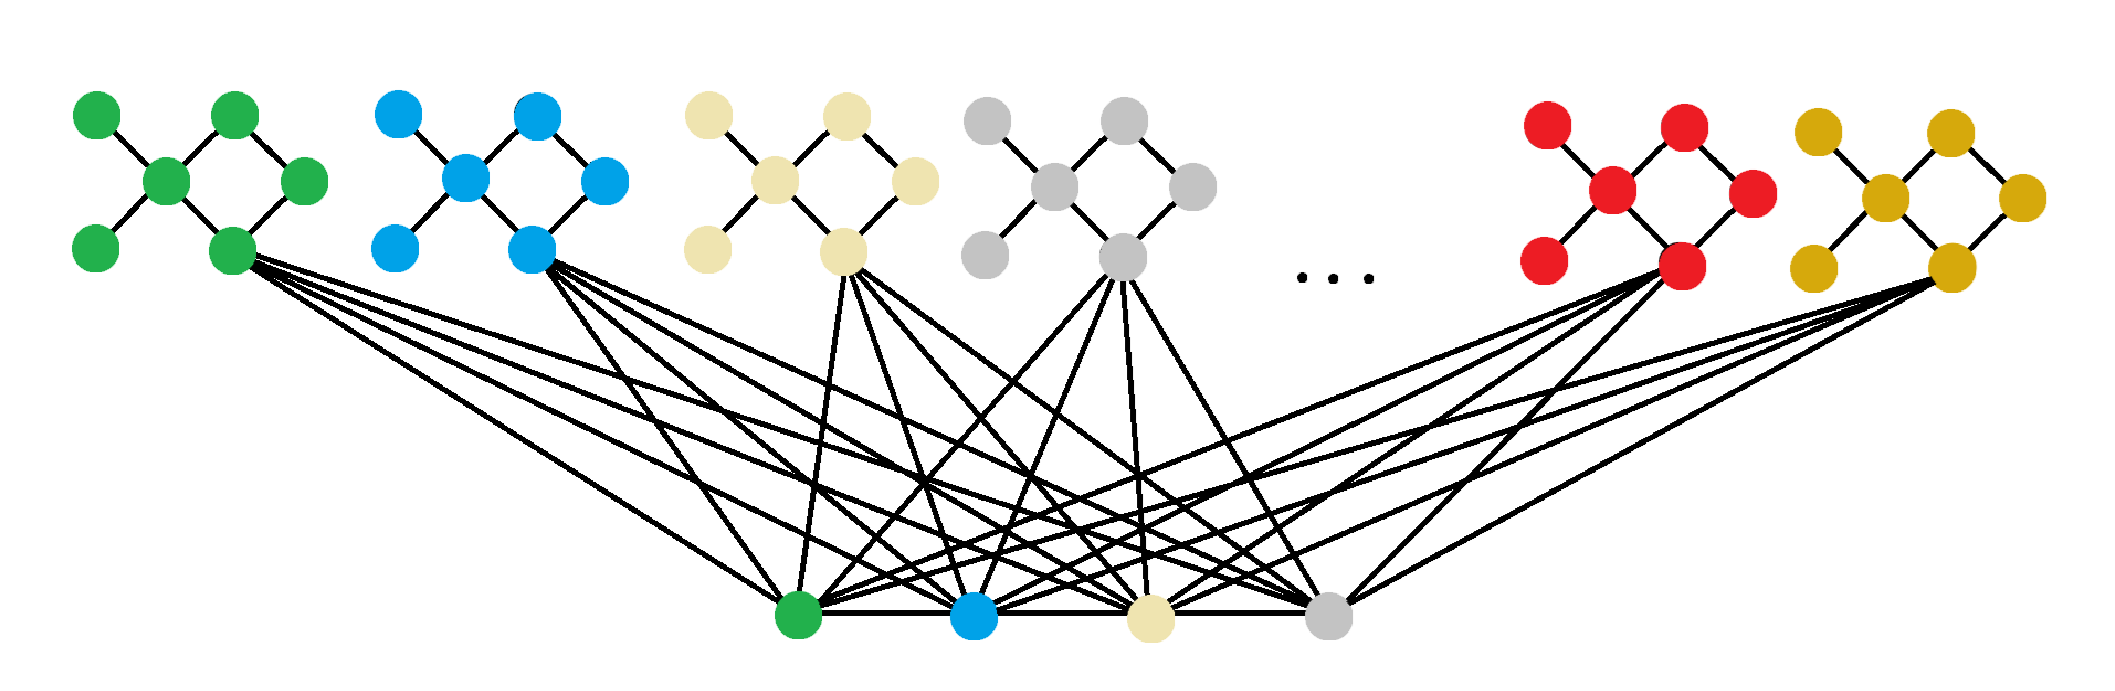
\includegraphics[width=0.99\textwidth]{../graphs/minus_mod.png}
  \caption{Graf ilustrujący hipotezę \ref{thesis_minus_mod}.}
  \label{fig:thesis_mod_star}
\end{figure}

Przedstawiony na powyższym rysunku graf \(G=(V,E)\), składa się z 500 \say{rybek} (każda \say{rybka} to graf składający się z \(S_4\) oraz dodatkowego wierzchołka połączonego z dwoma wierzchołkami gwiazdy innymi niż centralny) oraz ścieżki \(P_4\). Każdy wierzchołek \(P_4\) jest połączony z jednym, niecentralnym wierzchołkiem gwiazdy w każdej \say{rybce}.\\
Kolory przedstawiają społeczności partycji \(\mathcal{A}\), dla której \(mod_{\mathcal{A}}^*(G) \approx 0.491\). 496 społeczności składa się z pojedynczych \say{rybek}, a pozostałe 4 społeczności zawierają \say{rybkę} oraz jeden wierzchołek ścieżki. To właśnie te 4 społeczności kontrybuują ujemnie do modularity star score.\\

Jak dotąd nie udało się znaleźć partycji o wyższym modularity star score.\\
Rozpatrywane były partycjonowania m.in. takie jak:
\begin{itemize}
  \item każda \say{rybka} w osobnej społeczności, cała ścieżka w osobnej społeczności,
  \item 498 \say{rybek} w osobnych społecznościach, 2 społeczności zawierające po jednej \say{rybce} oraz 2 wierzchołki ścieżki,
  \item 4, 2 albo 1 społeczność zawierająca kilka \say{rybek} oraz odpowiednią liczbę wierzchołków ścieżki, reszta \say{rybek} w osobnych społecznościach.
  \item ścieżka (lub jej fragmenty) oraz wierzchołki o najwyższym stopniu z konkretnej liczby \say{rybek} w jednej społeczności, pozostałe części oraz reszta \say{rybek} w osobnych społecznościach.
\end{itemize}
W każdym z tych przypadków modularity star score okazywał się być mniejszy niż w przypadku partycji przedstawionej na rysunku powyżej.\\

\begin{conclusion}
  Jeśli hipoteza \ref{thesis_minus_mod} jest prawdziwa, to dodawanie izolowanych wierzchołków ma wpływ na modularity star grafu.
\end{conclusion}
Izolowane wierzchołki dodane do społeczności o ujemnym wkładzie zmniejszą ich star factor, przez co ich negatywny wpływ na modularity star grafu zmaleje.\\

\begin{conclusion}
  Niech \(G = (V,E)\) będzie grafem z co najmniej jedną krawędzią, \(\mathcal{A}\) partycją, dla której \(mod_{\mathcal{A}}^*(G) = mod^*(G)\). Wtedy, jeśli hipoteza \ref{thesis_minus_mod} jest prawdziwa, to nie wszystkie społeczności w partycji \(\mathcal{A}\) muszą indukować podgrafy spójne.\\
\end{conclusion}

\section{Modularity i modularity star grafów prawie pełnych}
W tym rozdziale przedstawimy odpowiedź na pytanie: Ile krawędzi należy usunąć z kliki, aby jej modularity oraz modularity star stały się niezerowe? Problem ten został poruszony i rozwiązany dla modularity w pracy \cite{MS23}. My uogólnimy go na modularity star.\\
\begin{fact}
  \label{clique_mod}
  Niech \(K_n\) będzie kliką o \(n\) wierzchołkach, \(n \geq 1\). Wtedy
  \[mod(K_n) = 0,\]
  \[mod^*(K_n) = 0.\]
\end{fact}

\begin{proof}
  Dla \(n=1\) mamy \(mod(K_1) = mod^*(K_1) = 0\), ponieważ graf nie zawiera krawędzi.\\
  Załóżmy więc, że \(n \geq 2\). Niech \(\mathcal{A} = \{A_1, A_2, \ldots, A_k\}\), \(k \leq n\) będzie k-elementową partycją zbioru wierzchołków \(K_n\), wtedy
  \begin{align*}
    mod_{\mathcal{A}}(K_n) & = \sum_{i=1}^k \left(\frac{\binom{|A_i|}{2}}{\binom{n}{2}} - {\left(\frac{|A_i|(n-1)}{n(n-1)}\right)}^2\right) \\
                           & = \sum_{i=1}^k \left(\frac{|A_i|(|A_i|-1)}{n(n-1)} - {\left(\frac{|A_i|}{n}\right)}^2\right)                   \\
                           & = \sum_{i=1}^k \frac{|A_i|^2 - n|A_i|}{n^2(n-1)}                                                               \\
                           & = \frac{\sum_{i=1}^k |A_i|^2 - n\sum_{i=1}^k |A_i|}{n^2(n-1)}                                                  \\
                           & = \frac{1}{n^2(n-1)} \cdot \sum_{i=1}^k |A_i|^2 - \frac{1}{n-1}.
  \end{align*}
  Zauważmy, że \(\forall_{A \in \mathcal{A}} \Delta(A) = |A| - 1\), co sprawia, że \(mod_{\mathcal{A}}(K_n) = mod_{\mathcal{A}}^*(K_n)\).\\
  Wartość \(mod_{\mathcal{A}}(K_n)\) jest maksymalna, gdy \(\sum_{i=1}^k |A_i|^2\) osiąga maksimum, a dzieje się to dla \(k=1\). (Przypomnijmy, że dla \(a,b>0\) mamy \((a+b)^2 \geq a^2 + b^2\)).\\

  Modularity score jednoelementowej partycji wynosi 0.\\
\end{proof}

\begin{conclusion}
  Dla każdego grafu \(G=(V, E)\) takiego, że \(|V| \leq 3\), \(mod(G) = mod^*(G) = 0\).\\
\end{conclusion}
Wniosek wynika z Faktu \ref{clique_mod} oraz własności przedstawionych w rozdziale \ref{własności}.\\

Zastanówmy się jednak jak dużo krawędzi trzeba z kliki usunąć, aby jej \(mod\) oraz \(mod^*\) były większe od zera.\\

\begin{fact}
  Dla każdej liczby naturalnej \(n \geq 4\) istnieje n-wierzchołkowy graf \(G\), taki że \(mod(G) > 0\) oraz \(mod^*(G) > 0\).\\
\end{fact}
\begin{proof}
  Wystarczy rozważyć ścieżkę \(P_n\) oraz partycję \(\mathcal{A}\) zbioru jej wierzchołków na dwie społeczności indukujące spójne podgrafy \(A_1\) i \(A_2\), gdzie \(|A_1| = \lceil\frac{n}{2}\rceil\) i \(|A_2| = \lfloor\frac{n}{2}\rfloor\).\\

  Jako pierwszy rozpatrzmy przypadek, gdy \(n\) jest liczbą parzystą. Wtedy
  \[mod_{\mathcal{A}}(P_n) = 2\cdot\left(\frac{\frac{n-2}{2}}{n-1} - {\left(\frac{1}{2}\right)}^2\right) = \frac{n-2}{n-1}-\frac{1}{2}=\frac{n-3}{2n-2}>0 \text{, dla } n \geq 4,\]
  \[mod_{\mathcal{A}}^*(P_n) = 2\cdot\left(\frac{\frac{n-2}{2}}{n-1} - {\left(\frac{1}{2}\right)}^2\right) \cdot \frac{3}{\frac{n}{2}}=\frac{n-3}{2n-2} \cdot \frac{6}{n} > 0\text{, dla } n \geq 4.\]

  Teraz załóżmy, że \(2\nmid n\).
  \begin{align*}
    mod_{\mathcal{A}}(P_n) & = \frac{\frac{n-1}{2}}{n-1} - {\left(\frac{\frac{n+1}{2}\cdot 2-1}{2(n-1)}\right)}^2 + \frac{\frac{n-3}{2}}{n-1} - {\left(\frac{\frac{n-1}{2}\cdot 2-1}{2(n-1)}\right)}^2 \\
                           & = \frac{4(n-1)(n-2)-2n^2+4n-4}{4(n-1)^2}                                                                                                                                  \\
                           & = \frac{n^2-4n+2}{2(n-1)^2}>0 \text{, dla } n \geq 4,
  \end{align*}
  \begin{align*}
    mod_{\mathcal{A}}^*(P_n) & \geq \left(\frac{\frac{n-1}{2}}{n-1} - {\left(\frac{\frac{n+1}{2}\cdot 2-1}{2(n-1)}\right)}^2\right) \cdot \frac{2}{\frac{n+1}{2}} + \left(\frac{\frac{n-3}{2}}{n-1} - {\left(\frac{\frac{n-1}{2}\cdot 2-1}{2(n-1)}\right)}^2\right) \cdot \frac{1}{\frac{n-1}{2}} \\
                             & = \frac{n^2-4n+2}{(n+1)(n-1)^2} + \frac{-1}{(n-1)^3}                                                                                                                                                                                                               \\
                             & = \frac{(n-1)(n^2-4n+2)}{(n+1)(n-1)^3}                                                                                                                                                                                                                             \\
                             & = \frac{n^2-4n+2}{(n+1)(n-1)^2}>0 \text{, dla } n \geq 4.
  \end{align*}
\end{proof}

Możemy zatem zdefiniować funkcję \textbf{\(f(n)\)}, która dla grafu \(K_n\) zwraca minimalną liczbę krawędzi, które należy usunąć, aby wartość modularity nowo otrzymanego grafu była większa od zera.\\

Analogicznie, niech \textbf{\(f^*(n)\)} będzie funkcją, która dla grafu \(K_n\) zwraca minimalną liczbę krawędzi, które należy usunąć, aby wartość modularity star nowo otrzymanego grafu była większa od zera.\\

\begin{lemma}
  \label{p_G'}
  Niech \(G = \left(V, E\right)\) będzie grafem z co najmniej jedną krawędzią. Niech \(A \subset V\) oraz \(G'\) będzie grafem powstałym z \(G\) poprzez usunięcie jednej krawędzi należącej do \(e(A, A^c)\) oraz dodanie jednej krawędzi do \(e(A)\) lub \(e(A^c)\). Wtedy
  \[p_{G'}(A) > p_G(A).\]
\end{lemma}
\begin{proof}
  Z lematu \ref{mod_eq} wiemy, że \(p_G(A) = p_G(A^c)\), więc załóżmy bez utraty ogólności, że krawędź dodajemy do \(e(A)\). Wtedy
  \(e_{G'}(A) = e_G(A)+1\), \(vol_{G'}(A) = vol_G(A) + 1\) oraz \(vol(G) = vol(G')\).\\
  Zatem
  \begin{align*}
    p_{G'}(A) - p_G(A) & \geq 2e_{G'}(A) \cdot vol(G') - vol_{G'}(A)^2 - \left(2e_{G}(A) \cdot vol(G) - vol_{G}(A)^2\right) \\
                       & = 2vol(G) - (vol_G(A)+1)^2 + vol_G(A)^2                                                            \\
                       & = 2vol(G) - 2vol_G(A) - 1 > 0.
  \end{align*}
\end{proof}
Lemat ten wykorzystamy w dowodzie twierdzenia \ref{f_star}.\\

\begin{theorem} %\cite[Theorem 1.1]{MS23}
  Dla każdej liczby naturalnej \(n \geq 4\), \(f(n) = \lfloor\frac{n}{2}\rfloor + 1\).
\end{theorem}

Poniżej przedstawimy analogiczne twierdzenie dla modularity star wraz z jego dowodem wzorowanym na dowodzie opisanym w pracy \cite{MS23}.\\

\begin{theorem}
  \label{f_star}
  Dla każdej liczby naturalnej \(n \geq 4\), \(f^*(n) = \lfloor\frac{n}{2}\rfloor + 1\).
\end{theorem}

\begin{proof}
  Niech \(G=(V,E)\) będzie grafem pełnym o \(n\) wierzchołkach. Niech \(\mathcal{A} = \{A_1, A_2\}\) będzie partycją \(V\), taką że \(|A_1| = \lceil\frac{n}{2}\rceil\) oraz \(|A_2| = \lfloor\frac{n}{2}\rfloor\). Niech \(k = \lfloor\frac{n}{2}\rfloor + 1\). Najpierw pokażemy, że po usunięciu \(k\) krawędzi spomiędzy \(A_1\) i \(A_2\), modularity star tak zmodyfikowanego grafu \(G'\) będzie większe od 0 - \(mod^*(G') > 0\). Zauważmy, że usunięcie krawędzi spomiędzy \(A_1\) i \(A_2\) nie wpływa na ich star factor - \(\rho(A_1) = \rho(A_2) = 1\).\\

  Jako pierwszy rozpatrzmy przypadek, gdy \(n\) jest liczbą parzystą. Wtedy \(k = \frac{n+2}{2}\).
  Liczba krawędzi w grafie \(G'\) jest równa \(m = \binom{n}{2} - k = \frac{n^2-2n-2}{2}\).

  \begin{align*}
    mod_\mathcal{A}^*(G') & = 2\cdot\left(\frac{\binom{\frac{n}{2}}{2}}{m} - {\left(\frac{1}{2}\right)}^2\right)      \\
                          & = \frac{1}{2}+\frac{1}{n^2-2n-2}-\frac{1}{2}=\frac{1}{n^2-2n-2}>0, \text{ dla } n \geq 4.
  \end{align*}


  Teraz załóżmy, że \(n\) jest liczbą nieparzystą. Wtedy \(k = \frac{n+1}{2}\). Liczba krawędzi w grafie \(G'\) jest równa \(m = \binom{n}{2} - k = \frac{n^2-2n-1}{2}\).

  \begin{align*}
    mod_\mathcal{A}^*(G') & = \left(\frac{\binom{\frac{n+1}{2}}{2}}{m} - {\left(\frac{\frac{n+1}{2}\cdot(n-1)-k}{2m}\right)}^2\right) + \left(\frac{\binom{\frac{n-1}{2}}{2}}{m} - {\left(\frac{\frac{n-1}{2}\cdot(n-1)-k}{2m}\right)}^2\right) \\
                          & = \frac{(n+1)(n-1)+(n-1)(n+3)}{8m} - \frac{(n^2-n-2)^2 + (n^2-3n)^2}{16m^2}                                                                                                                                         \\
                          & = \frac{(n-1)^2\cdot 2m}{8m^2} - \frac{n^4-4n^3+3n^2+2n+2}{8m^2}                                                                                                                                                    \\
                          & = \frac{(n+1)(n-3)}{8m^2} > 0 \text{, dla } n \geq 4.
  \end{align*}

  Pozostaje nam pokazać, że gdy usuniemy z grafu pełnego mniej niż \(\lfloor\frac{n}{2}\rfloor + 1\) krawędzi, to jego modularity star wciąż będzie równe 0.\\
  Z lematu \ref{mod_star_eq} wiemy, że wystarczy pokazać, że dla każdego niepustego podzbioru \(U \subset V\), \(p_G^*(U) \leq 0\). Przypomnijmy, że \(p_G^*(U)=p_G(U)\cdot \rho(U)=(2e(U)\cdot vol(G) - vol(U)^2)\cdot \rho(U)\).\\

  Niech graf \(G = (V, E)\) oraz podzbiór jego wierzchołków \(U\) będą takie, że wartość \(p_G(U)\) jest maksymalna pośród wszystkich grafów, w których do grafu pełnego brakuje co najwyżej \(\frac{n}{2}\) krawędzi oraz wszystkich niepustych podzbiorów jego wierzchołków. Ponieważ \(\frac{n}{2} < n-1\) oraz \(p_G(U)\) jest maksymalne, to podzbiory \(U\) oraz \(U^c\) są izomorficzne z grafami pełnymi oraz \(e(U, U^c) \neq 0\), co wynika z lematu \ref{p_G'}. Wiemy też, że \(\rho(U)=\rho(U^c)=1\), więc \(p_G^*(U)=p_G(U)\).\\

  Załóżmy, że \(|U| = j\), (\(1 \leq j \leq n-1\)) oraz w \(G\) do grafu pełnego brakuje \(x\) (\(\leq \frac{n}{2}\)) krawędzi. Wtedy
  \begin{align*}
    p_G^*(U) & = vol(U) \cdot vol(U^c) - e(U, U^c) \cdot vol(G)           \\
             & = (j(n-1) - x)((n-j)(n-1) - x) - (j(n-j) - x)(n(n-1) - 2x) \\
             & = (n-1)^2(n-j)j-xn(n-1)+x^2                                \\
             & - jn(n-j)(n-1)-2x^2+x(n(n-1)+2j(n-j))                      \\
             & = -j(n-j)(n-1) + 2xj(n-j) - x^2                            \\
             & = j(n-j)(2x-(n-1)) - x^2
  \end{align*}
  Widzimy zatem, że dla \(x \leq \frac{n-1}{2}\), \(p_G^*(U) \leq 0\). Gdy \(x = \frac{n}{2}\), to \(p_G^*(U) = j(n-j)-(\frac{n}{2})^2\). Czyli \(p_G^*(U)\) (a zatem także \(mod^*(G)\)) osiąga maksymalną wartość, równą \(0\), dla \(j = \frac{n}{2}\).

  Pokazaliśmy więc, że po usunięciu \(\lfloor\frac{n}{2}\rfloor + 1\) krawędzi z grafu pełnego \(K_n\), jego modularity star jest większe od 0 oraz, że po usunięciu z niego co najwyżej \(\frac{n}{2}\) krawędzi, jego modularity star wciąż wynosi 0.
\end{proof}

\section{Modularity i modularity star grafów prawie pełnych dwudzielnych}
W tym rozdziale zajmiemy się grafami pełnymi dwudzielnymi \(K_{s,t}\). Przypomnijmy, że graf pełny dwudzielny \(K_{s,t} = (S \cup T, E)\) to graf, którego zbiór wierzchołków można podzielić na dwa rozłączne zbiory \(S\) oraz \(T\), takie że \(|S| = s\), \(|T| = t\) oraz każda para wierzchołków \((u,v)\), gdzie \(u \in S\), \(v \in T\) jest połączona krawędzią i są to jedyne krawędzie w tym grafie.\\
Zastanowimy się, ile co najmniej krawędzi należy usunąć z grafu pełnego dwudzielnego \(K_{s,t}\), aby jego modularity oraz modularity star były większe od zera. Przypomnijmy, że oznaczamy te wartości odpowiednio jako \(\delta^{-}(K_{s,t})\) oraz \(\delta^{-}_*(K_{s,t})\).\\
W naszych rozważaniach pominiemy przypadek, gdy \(s = 1\) lub \(t = 1\), dla którego\\\(\delta^{-}=\delta^{-}_*=\infty\).
\begin{lemma}
  \label{sigma_tau}
  Niech \(K_{s,t} = (S\cup T, E)\) będzie grafem pełnym dwudzielnym takim, że \(2 \leq s \leq t\).~ Niech \(\mathcal{A} = \{A_1, A_2\}\) będzie partycją zbioru wierzchołków grafu \(K_{s,t}\), taką że \(e(A_1, A_2) > 0\) oraz niech \(\sigma = \frac{|A_1\cap S|}{s}\), \(\tau = \frac{|A_1 \cap T|}{t}\) będą proporcjami wierzchołków z \(S\) oraz \(T\) należących do społeczności \(A_1\) w partycji \(\mathcal{A}\). Wtedy
  \[mod_{\mathcal{A}}(K_{s,t}) = -\frac{1}{2}(\sigma-\tau)^2.\]
\end{lemma}

\begin{proof}
  Zauważmy, że
  \[e(A_1) = |A_1\cap S| \cdot |A_1\cap T| = \sigma s \cdot \tau t,\]
  \[e(A_2) = |A_2\cap S| \cdot |A_2\cap T| = (1-\sigma)s \cdot (1-\tau)t,\]
  \[vol(A_1) = |A_1\cap S| \cdot t + |A_1\cap T| \cdot s = (\sigma+\tau)st,\]
  \[vol(A_2) = |A_2\cap S| \cdot t + |A_2\cap T| \cdot s = ((1-\sigma)+(1-\tau))st = (2-\sigma-\tau)st.\]

  A zatem
  \begin{align*}
     & mod_{\mathcal{A}}(K_{s,t})                                                                                      \\
     & = \frac{e(A_1)+e(A_2)}{st} - \frac{vol(A_1)^2 + vol(A_2)^2}{4(st)^2}                                            \\
     & = \frac{st(\sigma \tau + (1-\sigma)(1-\tau))}{st} - \frac{((\sigma+\tau)st)^2 + ((2-\sigma-\tau)st)^2}{4s^2t^2} \\
     & = 1 - (\sigma + \tau) + 2\sigma \tau - (1-(\sigma+\tau) + \frac{(\sigma+\tau)^2}{2})                            \\
     & = 2\sigma \tau - \frac{(\sigma+\tau)^2}{2}                                                                      \\
     & = -\frac{(\sigma-\tau)^2}{2}.
  \end{align*}
\end{proof}

\begin{lemma}
  \cite[Theorem 3.1]{MS23}
  \label{bipartite_mod}
  Modularity oraz modularity star grafu pełnego dwudzielnego \(K_{s,t}\) są równe 0
  \[mod(K_{s,t}) = 0,\]
  \[mod(K_{s,t})^* = 0.\]
\end{lemma}

\begin{proof}
  Z lematów \ref{mod_eq} oraz \ref{mod_star_eq} wiemy, że wystarczy pokazać, że dla każdej partycji dwuelementowej \(\mathcal{A} = \{A_1, A_2\}\) zbioru wierzchołków grafu \(K_{s,t}\), \(mod_{\mathcal{A}}(K_{s,t})\) oraz \(mod_{\mathcal{A}}^*(K_{s,t})\) są mniejsze lub równe 0.\\
  Z lematów \ref{2partition} oraz \ref{2partition_star} mamy
  \[mod_{A_1}(K_{s,t}) = mod_{A_2}(K_{s,t}) = \frac{4e(A_1)e(A_2)-e(A_1,A_2)^2}{vol(K_{s,t})^2},\]
  \[mod^*_{A_1}(K_{s,t}) = \left(\frac{4e(A_1)e(A_2)-e(A_1,A_2)^2}{vol(K_{s,t})^2}\right) \rho(A_1),\]
  \[mod^*_{A_2}(K_{s,t}) = \left(\frac{4e(A_2)e(A_1)-e(A_2,A_1)^2}{vol(K_{s,t})^2}\right) \rho(A_2).\]

  A zatem musimy pokazać, że dla każdej partycji dwuelementowej \(\mathcal{A} = \{A_1, A_2\}\) zbioru wierzchołków grafu \(K_{s,t}\), zachodzi nierówność
  \[4e(A_1)e(A_2) \leq e(A_1,A_2)^2. \label{ineq} \tag{1}\]

  Korzystając z oznaczeń przedstawionych w lemacie \ref{sigma_tau} oraz tego, że \\\(e(A_1,A_2) = \sigma s (t-\tau t)+\tau t(s-\sigma s) = st(\sigma + \tau - 2\sigma \tau)\), możemy zapisać (\ref{ineq}) jako
  \begin{align*}
    4\sigma s \tau t \cdot (1-\sigma)s(1-\tau)t                          & \leq (s t (\sigma(1-\tau) + (1-\sigma)\tau))^2                                         \\
    4s^2t^2(\sigma \tau+\sigma^2 \tau^2 - \sigma^2 \tau - \sigma \tau^2) & \leq s^2t^2(\sigma^2 + \tau^2+4\sigma^2\tau^2+2\sigma\tau-4\sigma^2\tau-4\sigma\tau^2) \\
    4\sigma\tau                                                          & \leq \sigma^2 + \tau^2 + 2\sigma\tau                                                   \\
    (\sigma - \tau)^2                                                    & \geq 0.
  \end{align*}
  A zatem niezależnie od wyboru partycji dwuelementowej \(\mathcal{A} = \{A_1, A_2\}\) zbioru wierzchołków grafu \(K_{s,t}\), zachodzi nierówność (\ref{ineq}). Stąd wynika, że \(mod(K_{s,t}) = 0\) oraz \(mod^*(K_{s,t}) = 0\).
\end{proof}

\begin{lemma}
  \label{delete_edge}
  Niech \(\mathcal{A}=\{A_1, A_2\}\) będzie partycją zbioru wierzchołków grafu \(G\) o co najmniej 2 krawędziach, taką że \(mod_{\mathcal{A}}(G) \geq 0\) oraz \(e_G(A_1, A_2) > 0\). Niech \(G'\) będzie grafem powstałym z \(G\) poprzez usunięcie jednej krawędzi należącej do \(e_G(A_1, A_2)\). Wtedy \(mod_{\mathcal{A}}(G') > mod_{\mathcal{A}}(G)\).
\end{lemma}
\begin{proof}
  Z lematu \ref{2partition} wiemy, że
  \[mod_{\mathcal{A}}(G) = 2 \cdot \frac{4e(A_1)e(A_2)-e_G(A_1,A_2)^2}{vol(G)^2}\]
  oraz
  \[mod_{\mathcal{A}}(G') = 2 \cdot \frac{4e(A_1)e(A_2)-(e_G(A_1,A_2)-1)^2}{(vol(G)-2)^2}.\]

  Policzmy zatem różnicę
  \begin{align*}
     & mod_{\mathcal{A}}(G') - mod_{\mathcal{A}}(G)                                                                                     \\
     & = \frac{2 \left(\left(4e(A_1)e(A_2)-(e_G(A_1,A_2)-1)^2\right)\cdot vol(G)^2 \right)}{(vol(G)-2)^2 \cdot vol(G)^2}                \\
     & - \frac{2 \left(\left(4e(A_1)e(A_2)-e_G(A_1,A_2)^2\right)\cdot (vol(G)-2)^2\right)}{(vol(G)-2)^2 \cdot vol(G)^2}                 \\
     & = \frac{2\left(vol(G)^2\cdot2e_G(A_1,A_2)-vol(G)^2+16vol(G)e(A_1)e(A_2)\right)}{(vol(G)-2)^2 \cdot vol(G)^2}                     \\
     & + \frac{2\left(-16e(A_1)e(A_2)-4vol(G)e_G(A_1,A_2)^2+4e_G(A_1,A_2)^2\right)}{(vol(G)-2)^2 \cdot vol(G)^2}                        \\
     & = \frac{2\left(vol(G)^2(2e_G(A_1,A_2)-1)+16e(A_1)e(A_2)(vol(G)-1)+4e_G(A_1,A_2)^2(1-vol(G))\right)}{(vol(G)-2)^2 \cdot vol(G)^2} \\
     & = \frac{2\left(vol(G)^2(2e_G(A_1,A_2)-1)+4(vol(G)-1)(4e(A_1)e(A_2)-e_G(A_1,A_2)^2)\right)}{(vol(G)-2)^2 \cdot vol(G)^2}.
  \end{align*}
  Wiemy, że \(e_G(A_1,A_2) \geq 1\) oraz \(mod_{\mathcal{A}}(G) \geq 0\), zatem
  \[mod_{\mathcal{A}}(G') - mod_{\mathcal{A}}(G) > 0,\]
  co kończy dowód.
\end{proof}

Zatem, zgodnie z intuicją, usunięcie krawędzi spomiędzy dwóch społeczności zwiększa wartość modularity score danej partycji.\\

Dowód powyższego lematu przenosi się na modularity star, ponieważ wartości star factor obu społeczności pozostają bez zmian po usunięciu krawędzi pomiędzy nimi.

\begin{conclusion}
  Niech \(\mathcal{A}=\{A_1, A_2\}\) będzie partycją zbioru wierzchołków grafu \(G\) o co najmniej 2 krawędziach, taką że \(mod^*_{\mathcal{A}}(G) \geq 0\) oraz \(e_G(A_1, A_2) > 0\). Niech \(G'\) będzie grafem powstałym z \(G\) poprzez usunięcie jednej krawędzi należącej do \(e_G(A_1, A_2)\). Wtedy \(mod^*_{\mathcal{A}}(G') > mod^*_{\mathcal{A}}(G)\).\\
\end{conclusion}

% \begin{proof}
%   \[EC_{\mathcal{A}}(G) = \frac{e_G(A_1)+e_G(A_2)}{m}\]
%   \[EC_{\mathcal{A}}(G') = \frac{e_G(A_1)+e_G(A_2)}{m-1}\]

%   Niech \(q = vol_G(A_1)-m = m-vol_G(A_2)\). Wtedy:
%   \[DT_{\mathcal{A}}(G) = \frac{(m+q)^2 + (m-q)^2}{4m^2} = \frac{m^2+q^2}{2m^2}\]
%   \[DT_{\mathcal{A}}(G') = \frac{(m+q-1)^2 + (m-q-1)^2}{4(m-1)^2} = \frac{m^2+q^2+1-2m}{2(m-1)^2}\]

%   Zatem:
%   \[EC_{\mathcal{A}}(G)-EC_{\mathcal{A}}(G') = \frac{e_G(A_1)+e_G(A_2)}{m(m-1)}\]
%   \[DT_{\mathcal{A}}(G)-DT_{\mathcal{A}}(G') = \frac{q^2(1-2m)}{2m^2(m-1)^2}\]
%   \begin{align*}
%     mod_{\mathcal{A}}(G') - mod_{\mathcal{A}}(G)\\
%     &= \frac{e_G(A_1)+e_G(A_2)}{m(m-1)} - \frac{q^2(2m-1)}{2m^2(m-1)^2}\\
%     &= \frac{(e_G(A_1)+e_G(A_2))(2m(m-1)) - q^2(2m-1)}{2m^2(m-1)^2}
%   \end{align*}

%   Wiemy, że \(mod_{\mathcal{A}}(G) \geq 0\), zatem:
%   \[\frac{e_G(A_1)+e_G(A_2)}{m} = EC(G) \geq DT(G) = \frac{m^2+q^2}{2m^2}\]
%   \[2m(e_G(A_1)+e_G(A_2)) \geq (m^2+q^2)\]

%   Czyli:
%   \begin{align*}
%     mod_{\mathcal{A}}(G') - mod_{\mathcal{A}}(G)\\
%     &\geq \frac{(m^2+q^2)(m-1)- q^2(2m-1)}{2m^2(m-1)^2}\\
%     &= \frac{m^3-m^2-mq^2}{2m^2(m-1)^2}
%   \end{align*}

%   Wiemy, że \(0 \leq q \leq m-1\) (\(e_G(A_1, A_2) > 0\)). Zatem:
%   \[m^3-m^2-mq^2 \geq m^3-m^2-m(m-1)^2 = m(m-1) > 0\]
%   oraz:
%   \[mod_{\mathcal{A}}(G') - mod_{\mathcal{A}}(G) \geq \frac{m(m-1)}{2m^2(m-1)^2} = \frac{1}{2m(m-1)} \geq 0\]
% \end{proof}

\begin{theorem}
  \cite[Lemma 2.3]{MS23}
  Niech \(K_{s,t}=(S \cup T, E)\) będzie grafem pełnym dwudzielnym, gdzie \(2 \leq s \leq t\). Wtedy
  \[\delta^-(K_{s,t}) = 1.\]
\end{theorem}
\begin{proof}
  Z lematu \ref{bipartite_mod} wiemy, że \(mod(K_{s,t}) = 0\). Pokażemy, że po usunięciu jednej krawędzi z \(K_{s,t}\), jego wartość modularity stanie się większa od zera.\\

  Niech \(\mathcal{A} = \{A_1, A_2\}\) będzie partycją zbioru wierzchołków grafu \(K_{s,t}\), taką że \(e(A_1, A_2) > 0\) oraz niech \(\sigma = \frac{|A_1\cap S|}{s}\), \(\tau = \frac{|A_1 \cap T|}{t}\) będą proporcjami wierzchołków z \(S\) oraz \(T\) należących do społeczności \(A_1\) w partycji \(\mathcal{A}\).\\

  Rozpatrzymy dwa przypadki.
  \begin{enumerate}
    \item Przypadek, gdy \(s\) i \(t\) mają wspólny dzielnik.\\
          Naszym celem jest znalezienie partycji \(\mathcal{A} = \{A_1, A_2\}\) takiej, że \(e(A_1, A_2) > 0\) oraz \(mod_{\mathcal{A}} = 0\) (z lematu \ref{sigma_tau}: \(\sigma = \tau\)). Wtedy z lematu \ref{delete_edge} wynika, że usunięcie jednej krawędzi spomiędzy \(A_1\) i \(A_2\) spowoduje wzrost wartości modularity score, a zatem będzie ona dodatnia.\\

          Niech \(l\) będzie wspólnym dzielnikiem \(s\) oraz \(t\). Wtedy możemy dobrać \(\sigma = \tau = \frac{1}{l}\).\\
          Z lematu \ref{sigma_tau} mamy
          \[mod_{\mathcal{A}}(K_{s,t}) = -\frac{1}{2}\left(\frac{1}{l}-\frac{1}{l}\right)^2 = 0,\]
          co kończy dowód w tym przypadku.
    \item Przypadek, gdy \(s\) oraz \(t\) są względnie pierwsze.\\
          Niech \(K_{s,t}'\) będzie grafem powstałym z \(K_{s,t}\) poprzez usunięcie jednej krawędzi spomiędzy \(A_1\) i \(A_2\).\\
          Wtedy
          \[mod_{\mathcal{A}}(K_{s,t})= \frac{e(A_1)+e(A_2)}{e(K_{s,t})}-\frac{vol(A_1)^2+vol(A_2)^2}{4e(K_{s,t})^2},\]
          \[mod_{\mathcal{A}}(K_{s,t}')= \frac{e(A_1)+e(A_2)}{e(K_{s,t})-1}-\frac{(vol(A_1)-1)^2+(vol(A_2)-1)^2}{4(e(K_{s,t})-1)^2}.\]

          A zatem
          \begin{align*}
             & (e(K_{s,t})-1)^2 \cdot mod_{\mathcal{A}}(K_{s,t}')                                           \\
             & = e(K_{s,t})^2 \cdot mod_{\mathcal{A}}(K_{s,t})-e(A_1)-e(A_2)+2vol(A_1)+2vol(A_2)-2          \\
             & = e(K_{s,t})^2 \cdot mod_{\mathcal{A}}(K_{s,t})-e(A_1)-e(A_2)+4(e(A_1)+e(A_1, A_2)+e(A_2))-2 \\
            % &= e(K_{s,t})^2 \cdot mod_{\mathcal{A}}(K_{s,t}) + 3(e(A_1)+e(A_2))+4e(A_1, A_2) - 2\\
            % &= e(K_{s,t})^2 \cdot mod_{\mathcal{A}}(K_{s,t}) + 3e(K_{s,t})+e(A_1,A_2)-2\\
             & = e(K_{s,t})^2 \cdot mod_{\mathcal{A}}(K_{s,t}) + 4e(K_{s,t})-e(A_1)-e(A_2)-2.
          \end{align*}

          Korzystając z lematu \ref{sigma_tau}, otrzymujemy
          \begin{align}
             & (e(K_{s,t})-1)^2 \cdot mod_{\mathcal{A}}(K_{s,t}') \notag                                           \\
             & = s^2t^2 \cdot (-\frac{(\sigma-\tau)^2}{2}) + 4st - 2 - st(\sigma \tau + (1-\sigma)(1-\tau)) \notag \\
             & = -s^2t^2 \frac{(\sigma-\tau)^2}{2} + st(3 + \sigma + \tau - 2\sigma \tau) - 2 \notag               \\
             & = -s^2t^2 \frac{(\sigma-\tau)^2}{2} + st(3 + \sigma - \tau + 2\tau(1 - \sigma)) - 2. \label{modK}
          \end{align}

          Zauważmy, że jeśli \(s\) oraz \(t\) są względnie pierwsze, to równanie \(at - bs = 1\) ma rozwiązanie \((a,b)\) w liczbach całkowitych. Ale skoro \((a,b)\) jest rozwiązaniem, to \((a+s, b+t)\) również. Możemy zatem znaleźć takie \((a',b')\), że \(a't - b's = 1\) oraz \(1 \leq a' \leq s-1\).\\
          Wtedy \(t-1 \leq b's = a't-1 \leq (s-1)t-1\).\\
          Wiemy, że \(t-1 > 0\), więc \(b' > 0\) oraz \(b's \leq st-t-1\), więc \(b' < t\).\\
          Mamy zatem \((a',b')\) takie, że
          \[1 \leq a' \leq s-1,\]
          \[1 \leq b' \leq t-1,\]
          \[a't - b's = 1.\]

          Dobierzmy teraz \(\sigma = \frac{a'}{s}\) oraz \(\tau = \frac{b'}{t}\).\\
          Wtedy
          \[|\sigma - \tau| = |\frac{a'}{s} - \frac{b'}{t}| = \frac{|a't - b's|}{st} = \frac{1}{st}.\]

          Podstawiając do równania (\ref{modK}), otrzymujemy
          \begin{align*}
             & (e(K_{s,t})-1)^2 \cdot mod_{\mathcal{A}}(K_{s,t}')                                  \\
             & = -s^2t^2 \frac{(\frac{1}{st})^2}{2} + st(3 + \frac{1}{st} + 2\tau(1 - \sigma)) - 2 \\
             & = -\frac{3}{2} + 3st + 2st\tau(1 - \sigma)                                          \\
             & \geq -\frac{3}{2} + 3\cdot 4 > 0.
          \end{align*}

          Otrzymaliśmy \((e(K_{s,t})-1)^2 \cdot mod_{\mathcal{A}}(K_{s,t}') > 0\), czyli \(mod_{\mathcal{A}}(K_{s,t}') > 0\). Zatem po usunięciu jednej krawędzi z grafu pełnego dwudzielnego wartość jego modularity staje się większa od zera.
  \end{enumerate}
\end{proof}

Zauważmy, że dowód powyższego twierdzenia przenosi się na modularity star, ponieważ wartości star factor obu społeczności pozostają bez zmian po usunięciu krawędzi pomiędzy nimi.\\
A zatem prawdziwe jest następujące twierdzenie.
\begin{theorem}
  \label{delta_star}
  Niech \(K_{s,t}=(S \cup T, E)\) będzie grafem pełnym dwudzielnym, gdzie \(2 \leq s \leq t\). Wtedy
  \[\delta^{-}_*(K_{s,t}) = 1.\]
\end{theorem}

% I w tym momencie pojawia się ważne (wciąż otwarte) pytanie:
% \[\text{Czy dla każdego grafu $G$ } mod^*(G) \leq mod(G)?\]

\section{Pytanie otwarte}
Pytaniem otwartym wciąż pozostaje, czy dla każdego grafu \(G\) \(mod^*(G) \leq mod(G)\)?\\
Naszym zdaniem niekoniecznie. Poniżej przedstawiamy argumentację przemawiającą za tym, że możliwe jest istnienie grafu \(G\), dla którego \(mod^*(G) > mod(G)\).\\

Oczywiście partycja maksymalizująca \(mod(G)\) (nazwijmy ją \(\mathcal{B}\)) musi być różna od tej, która maksymalizuje \(mod^*(G)\) (nazwijmy ją \(\mathcal{A}\)). Zatem w grafie \(G\) musi istnieć partycjonowanie \(\mathcal{A}\), w którym wartość modularity score, co najmniej jednej społeczności (nazwijmy ją \(A\)), jest mniejsza od 0 i jednocześnie jej star factor jest mniejszy od 1. Jeśli pozostałe społeczności osiągną wystarczająco wysokie modularity score, to może się okazać, że dzięki zmniejszeniu bezwzględnej wartości \(mod_A(G)\) (poprzez star factor), \(mod^*_{\mathcal{A}}(G) > mod(G)\).\\

Dla grafu \(G\), o strukturze opisanej poniżej, nie znaleziono dotychczas partycjonowania, dla którego wartość modularity score byłaby większa od maksymalnej znalezionej dotychczas wartości modularity star score dla tego grafu: \(0.5511554446465\).\\

Graf \(G\) składa się z 9000 \say{diamentów} (każdy \say{diament} to graf powstały z gwiazdy \(S_3\) poprzez dodanie dwóch krawędzi pomiędzy jej liśćmi) oraz ścieżki \(P_4\). W każdym \say{diamencie} istnieje dokładnie jeden wierzchołek (o stopniu 2 w \say{diamencie}), który jest połączony z każdym wierzchołkiem ścieżki.\\

Graf G został przedstawiony na rysunku \ref{mod_star}. Kolory przedstawiają poszczególne społeczności partycji \(\mathcal{A}\), dla której \(mod_{\mathcal{A}}^*(G) \approx 0.5511554446465\). 8988 społeczności składa się z pojedynczych \say{diamentów}, a pozostałe 4 społeczności zawierają 3 \say{diamenty} oraz 1 wierzchołek ścieżki. To właśnie te 4 społeczności kontrybuują ujemnie do modularity star score.

\begin{figure}[H]
  \centering
  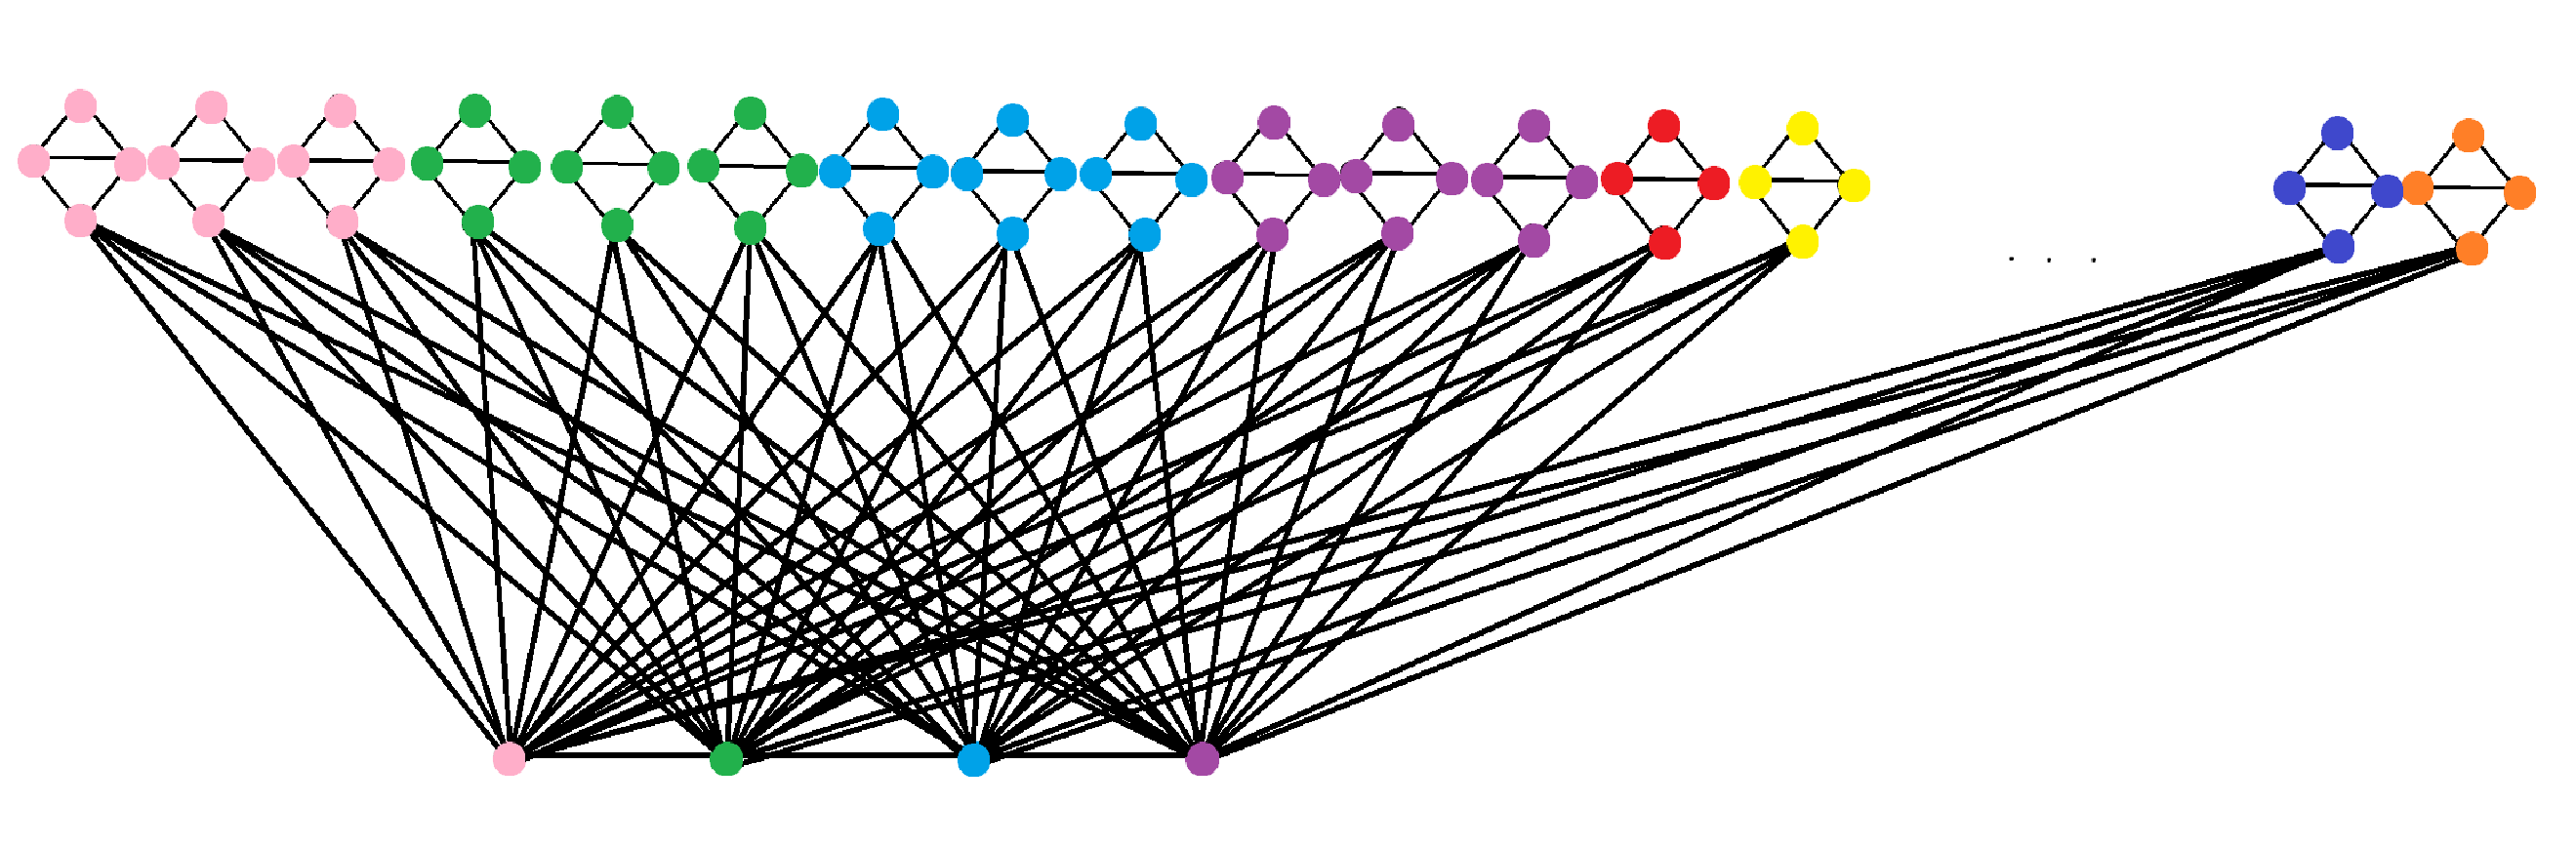
\includegraphics[width=0.99\textwidth]{../graphs/mod_star.png}
  \caption{Graf \(G\), dla którego hipotetycznie \(mod^*(G) > mod(G)\).}
  \label{mod_star}
\end{figure}

Należy zwrócić uwagę na fakt, że do partycji, w której istnieje społeczność kontrybuująca ujemnie, możemy dodać izolowane wierzchołki powodując wzrost wartości modularity star score. W ten sposób jeszcze bardziej zwiększamy różnicę pomiędzy modularity star a modularity.\\

Ścieżka w grafie \(G\) jest strukturą, która obniża jego modularity. Dodając jednak izolowane wierzchołki (co nie wpływa na modularity) możemy zminimalizować negatywny wpływ ścieżki na modularity star. Oznacza to, że być może dla grafu \(G\) z izolowanymi wierzchołkami \(mod^*(G) > mod(G)\).\\

Największa znaleziona dotychczas wartość modularity score dla tego grafu to około \\ \(0.54413127767\). Jest ona osiągana dla partycji, w której 4 społeczności zawierają po 184 \say{diamenty} oraz 1 wierzchołek ścieżki, a pozostałe 8264 \say{diamenty} są w osobnych społecznościach. Każda ze społeczności w tej partycji ma dodatni wkład do modularity score, co jest warunkiem koniecznym do tego, aby było to optymalne partycjonowanie dla modularity.\\

% \section{Brudnopis}
%   Analizowałam grafy \(G\), które w swojej strukturze zawierały:
%   \begin{itemize}
%     \item pewną liczbę klik lub gwiazd (również z dodatkowymi krawędziami) (\(\mathcal{T} = \{
%       T_1, T_2, \ldots, T_k\}\)) jako podgrafy indukowane,
%     \item pewną liczbę cykli lub ścieżek (\(\mathcal{H} = \{H_1, H_2, \ldots, H_l\}\)) jako podgrafy indukowane,
%     \item pewną liczbę krawędzi pomiędzy \(T \in \mathcal{T}\) a \(H \in \mathcal{H}\).
%   \end{itemize}

%   Udało mi się znaleźć takie grafy i ich partycjonowania, że \(mod^*(G)\) było minimalnie mniejsze niż \(mod(G)\). Wraz ze wzrostem liczebności \(\mathcal{T}\), różnica się zmniejsza. Niestety, wydaje się jednak, że w ten sposób nie dojdziemy do momentu, w którym się odwróci, ponieważ wraz ze zmniejszaniem różnicy pomiędzy \(mod^*_{\mathcal{A}}(G)\) a \(mod_{\mathcal{B}}(G)\) maleje również różnica pomiędzy \(mod^*_{\mathcal{A}}(G)\) a \(mod_{\mathcal{A}}(G)\). A kiedy ta różnica stanie się \(\leq 0\), to nasze rozważania tracą sens.\\

%   Udało mi się zauważyć pewną zależność pomiędzy \(|\mathcal{T}|\) a \(|T|\).\\

%   Niech \(\mathcal{A}\) partycjonuje \(G\) w taki sposób, że każdy element \(\mathcal{T} \cup \mathcal{H}\) stanowi osobną społeczność oraz niech \(\forall_{i \in \{1, \ldots k\}} T_i \cong S_m\) i \(\mathcal{H} = \{C_4\}\).\\

%   Wtedy dla \(m = k+1\) mamy \(mod^*_{\mathcal{A}}(G) = mod_{\mathcal{A}}(G)\) (a najprawdopodobniej również \(= mod(G)\)).\\
%   Jest to wynikiem zerowej wartości \textit{modularity\_score} dla \(A\).\\


%   Jeśli jednak \(\mathcal{H} = \{C_5\}\), to równość \(mod^*_{\mathcal{A}}(G) = mod_{\mathcal{A}}(G)\) zachodzi dla \(m = k+\frac{k}{4}+1\) dla \(4|k\).

%   Czy można z tego wyciągnąć sensowne wnioski na temat (nie)istnienia grafu \(G\) takiego, że \(mod^*(G) > mod(G)\)?\\

%   Oznaczenia:
%   \begin{itemize}
%     \item \(\delta^{-}(G)\) - minimalna liczba krawędzi, które należy usunąć z grafu \(G\), aby \(mod(G) > 0\).
%     \item \(\delta^{+}(G)\) - minimalna liczba krawędzi, które należy dodać do grafu \(G\), aby \(mod(G) > 0\).
%     \item \(\delta(G)\) - minimalna liczba krawędzi, które należy dodać lub usunąć z grafu \(G\), aby \(mod(G) > 0\).
%   \end{itemize}
%   Niech \(G\) będzie grafem pełnym dwudzielnym \(K_{s,t}\) (\(s \leq t\)) oraz niech \(\mathcal{A}\) będzie partycją zbioru wierzchołków \(G\) przedstawioną na schematach poniżej.\\

%   \begin{enumerate}[label=(\alph*)]
%     \item Jeśli \(s > 1\), to \(\delta^{-}(G) = 1\).
%     \begin{figure}[H]
%       \centering
%       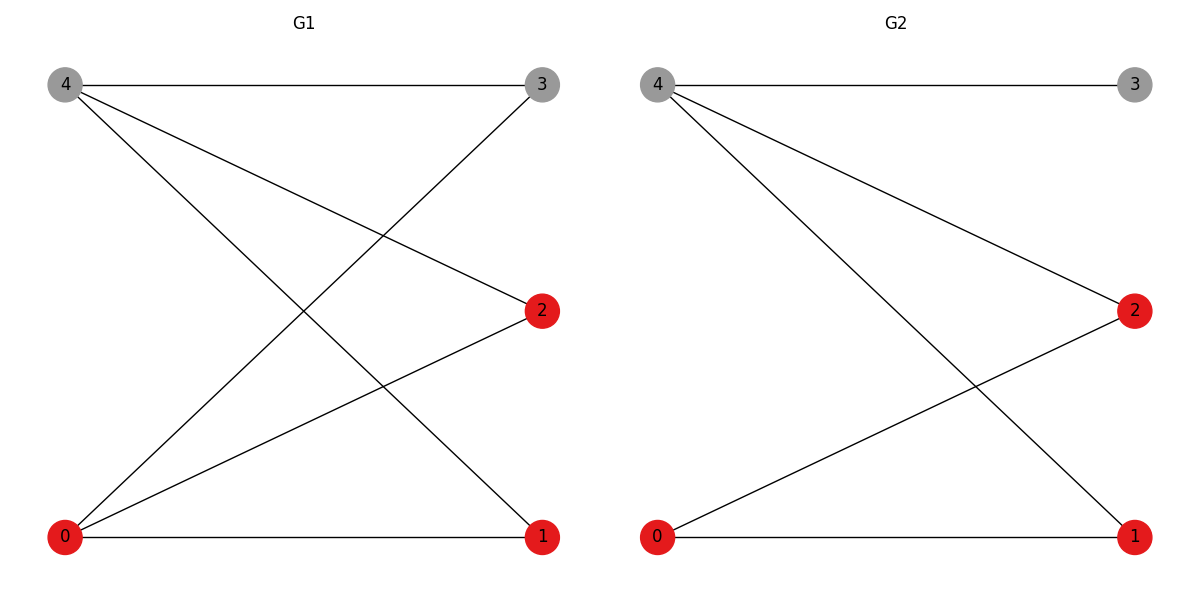
\includegraphics[width=0.6\textwidth]{../graphs/th1_3a.png}
%       \label{fig:th1_3a}
%     \end{figure}
%     \(mod_{\mathcal{A}}(G1) = -0.0138888889\), \(mod(G2) = 0.08\)

%     \item Jeśli \(s = 1\) i \(t \geq 4\) oraz \(s \geq 2\) i \(t \geq 3\) to \(\delta^{+}(G) = 1\). W pozostałych przypadkach \(\delta^{+}(G) = \infty\).
%     \begin{figure}[H]
%       \centering
%       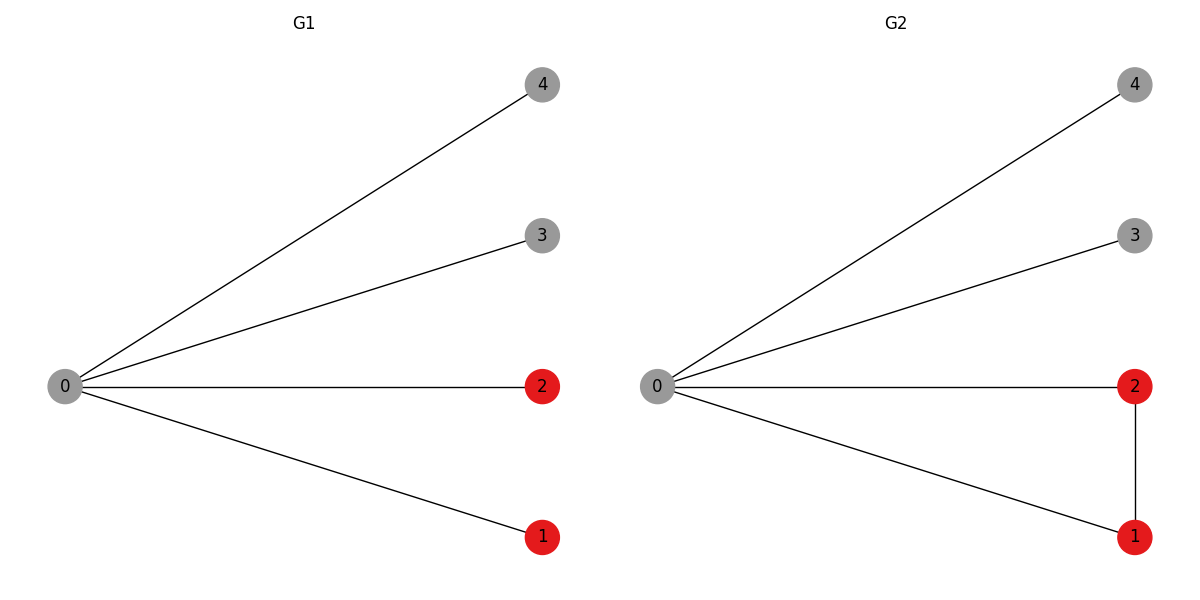
\includegraphics[width=0.6\textwidth]{../graphs/th1_3b.png}
%       \label{fig:th1_3b}
%     \end{figure}
%     \(mod_{\mathcal{A}}(G1) = -0.125\), \(mod(G2) = 0.08\)
%     \begin{figure}[H]
%       \centering
%       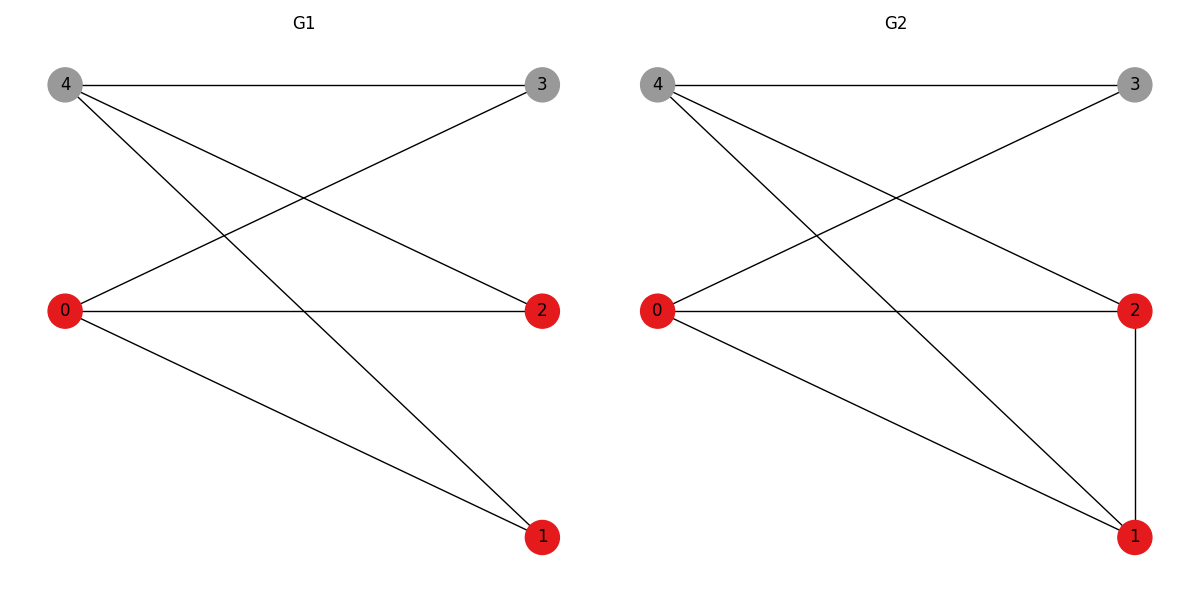
\includegraphics[width=0.6\textwidth]{../graphs/th1_3bb.png}
%       \label{fig:th1_3bb}
%     \end{figure}
%     \(mod_{\mathcal{A}}(G1) = -0.0138888889\), \(mod(G2) = 0.0306122449\)
%     \item Jeśli \(s = 1\) i \(t \geq 4\) albo \(s \geq 2\), to \(\delta(G) = 1\). Jeśli (s,t) = (1,2), to \(\delta(G) = \infty\). A gdy (s,t) = (1,3), to \(\delta(G) = 2\).
%   \end{enumerate}



% \begin{proof}
%   Niech \(\mathcal{A} = \{A_1, A_2, \ldots, A_t\}\) będzie partycją zbioru wierzchołków \(G\), dla której \(mod_{\mathcal{A}}^*(G) = mod^*(G)\).\\

%   Rozpatrzmy trzy przypadki.
%   \begin{enumerate}
%     \item Przypadek \(t=1\).\\
%     Jeśli optymalna partycja składa się z jednej społeczności, to modularity star grafu \(G\) jest równe 0. Wtedy nierówność z twierdzenia jest spełniona, gdyż obie jej strony są równe 0.
%     \item Przypadek \(t=2\).\\
%     Jeśli optymalna partycja składa się z dwóch społeczności, to \(mod_{\mathcal{A}}^*(G) = mod^*(G)\). Wtedy nierówność z tezy twierdzenia możemy zapisać jako
%     \[mod_{\mathcal{A}}^*(G) \leq \frac{2\rho_{max}(\mathcal{A})}{\rho_{min}(\mathcal{A})} \cdot mod_{\mathcal{A}}^*(G).\]\\
%     Oczywiście \(\rho_{min}(\mathcal{A}) \leq \rho_{max}(\mathcal{A})\), a zatem nierówność jest spełniona.
%     \item Przypadek \(t>2\).\\
%     Wiemy, że modularity star score partycji jednoelementowej wynosi 0, więc stwórzmy partycję \(\mathcal{B} = \{B_1, B_2\}\) poprzez pogrupowanie społeczności z \(\mathcal{A}\) w zbiory \(B_1, B_2\) (niekoniecznie oba niepuste). Dla każdej społeczności \(A_i \in \mathcal{A}\) wybieramy jednostajnie losowo i niezależnie społeczność \(B_1\) lub \(B_2\) i dodajemy do niej \(A_i\).\\
%     Z lematu \ref{score_deg_star} wiemy, że modularity star score partycji \(\mathcal{A}\) jest równe
%     \[
%       mod_{\mathcal{A}}^*(G) = \frac{1}{vol(G)} \cdot \sum_{\substack{u,v \in V \\ X_{uv}=1}} \left(\mathbbm{1}_{\{u,v\} \in E} - \frac{deg_G(u) \cdot deg_G(v)}{vol(G)}\right)\cdot \rho(A_{uv}),
%     \]
%     gdzie
%     \[
%       X_{uv} = \begin{cases}
%         1 & \text{jeśli } u \text{ i } v \text{ należą do tej samej społeczności w } \mathcal{A}, \\
%         0 & \text{w przeciwnym razie.}
%       \end{cases},
%     \]
%     \[A_{uv} - \text{społeczność } \mathcal{A} \text{, do której należą wierzchołki } u \text{ oraz } v.\]\\
%     Oznaczmy przez \(C_{u,v} = \mathbbm{1}_{\{u,v\} \in E} - \frac{deg_G(u) \cdot deg_G(v)}{vol(G)}\).\\
%     W celu uproszczenia zapisu poprzez \(\sum_{X_{uv} = 0}\) będziemy rozumieć \(\sum_{\substack{u,v \in V \\\land X_{uv} = 0}}\). Analogicznie dla \(X_{uv}=1\).\\
%     Teraz modularity score partycji \(\mathcal{A}\) możemy zapisać jako
%     \[
%       mod_{\mathcal{A}}^*(G) = \frac{1}{vol(G)} \cdot \sum_{X_{uv} = 1}\left(C_{u,v} \cdot \rho(A_{uv})\right).
%     \]

%     Zastanówmy się nad wartością oczekiwaną \(\mathbb{E}[mod_{\mathcal{B}}^*(G)]\).
%     \begin{itemize}
%       \item Jeśli \(X_{uv} = 1\), to \(u\) i \(v\) należą do tej samej społeczności w \(\mathcal{A}\), więc należą do tej samej społeczności również w \(\mathcal{B}\) - wkład \(C_{u,v}\) zostanie policzony (z inną wartością star factor).
%       \item Jeśli \(X_{uv} = 0\), to \(u\) i \(v\) należą do różnych społeczności w \(\mathcal{A}\), to z prawdopodobieństwem \(\frac{1}{2}\) trafią do tej samej społeczności w \(\mathcal{B}\) - wkład \(C_{u,v}\) zostanie pomnożony przez \(\frac{1}{2}\) (oraz star factor nowej społeczności z \(\mathcal{B}\)).
%     \end{itemize}
%   Zatem
%   \[\mathbb{E}[mod_{\mathcal{B}}^*(G)] = \frac{1}{vol(G)} \cdot \left(\sum_{X_{uv} = 1} (C_{u,v}\cdot \rho(B_{uv})) + \frac{1}{2}\sum_{X_{uv} = 0} (C_{u,v} \cdot \rho(B_{uv}))\right).\]\\

%   Zauważmy, że \(\sum_{u,v \in V} C_{u,v} = 0\), ponieważ dla partycji jednoelementowej \(\mathcal{T}\)\\ \(mod_{\mathcal{T}}(G) = \frac{1}{vol(G)} \cdot \sum_{u,v \in V} C_{u,v} = 0\).\\
%     Zatem
%     \[\sum_{X_{uv} = 1} C_{u,v} + \sum_{X_{uv} = 0} C_{u,v} = 0,\]
%     \[\sum_{X_{uv} = 0} C_{u,v} = -\sum_{X_{uv} = 1} C_{u,v}.\]

%     Niech \( \mathcal{A}_1, \mathcal{A}_2 \subseteq \mathcal{A}\) takie, że
%     \begin{itemize}
%       \item[-] \(\mathcal{A}_1 = \{A_i \in \mathcal{A} : mod_{A_i}^*(G) < 0\},\)
%       \item[-] \(\mathcal{A}_2 = \{A_i \in \mathcal{A} : mod_{A_i}^*(G) \geq 0\}.\)
%     \end{itemize}
%     Czyli
%     \[
%       mod_{\mathcal{A}}^*(G) \leq \frac{\rho_{min}(\mathcal{A})}{vol(G)} \cdot \sum_{\substack{X_{uv} = 1 \\ A_{uv} \in \mathcal{A}_1}}C_{u,v} + \frac{\rho_{max}(\mathcal{A})}{vol(G)} \cdot \sum_{\substack{X_{uv} = 1 \\ A_{uv} \in \mathcal{A}_2}}C_{u,v}.
%     \]

%     Niech \(\mathcal{B'} = argmax_{\mathcal{B}: |\mathcal{B}|\leq 2} mod_{\mathcal{B}}^*(G)\). Wobec tego wartość oczekiwana \(mod_{\mathcal{B}}^*(G)\) jest ograniczona z dołu przez
%     \begin{align*}
%       &\mathbb{E}[mod_{\mathcal{B}}^*(G)] = \frac{1}{vol(G)} \cdot \left(\sum_{X_{uv} = 1} (C_{u,v}\cdot \rho(B_{uv})) +  \frac{1}{2}\sum_{X_{uv} = 0} (C_{u,v} \cdot \rho(B_{uv}))\right)\\ \tag{1} \label{bound}
%       &\geq \frac{1}{vol(G)} \cdot \rho_{min}(\mathcal{B'}) \cdot \left(\sum_{X_{uv} = 1} C_{u,v} - \sum_{X_{uv} = 1} C_{u,v} \cdot \frac{1}{2}\right)\\
%       &= \frac{1}{2vol(G)} \cdot \rho_{min}(\mathcal{B'}) \cdot \sum_{X_{uv} = 1} C_{u,v}\\
%       &= \frac{1}{2vol(G)} \cdot \rho_{min}(\mathcal{B'}) \cdot \left(\sum_{\substack{X_{uv} = 1 \\ A_{uv} \in \mathcal{A}_1}} C_{u,v} + \sum_{\substack{X_{uv} = 1 \\ A_{uv} \in \mathcal{A}_2}} C_{u,v}\right)\\
%       &= \frac{1}{2vol(G)} \cdot \frac{\rho_{min}(\mathcal{B'})}{\rho_{min}(\mathcal{A})} \cdot \rho_{min}(\mathcal{A}) \cdot \sum_{\substack{X_{uv} = 1 \\ A_{uv} \in \mathcal{A}_1}} C_{u,v}\\
%       &+ \frac{1}{2vol(G)} \cdot \frac{\rho_{min}(\mathcal{B'})}{\rho_{max}(\mathcal{A})} \cdot \rho_{max}(\mathcal{A}) \cdot \sum_{\substack{X_{uv} = 1 \\ A_{uv} \in \mathcal{A}_2}} C_{u,v}\\
%       &\geq \frac{\rho_{min}(\mathcal{B'})}{2\rho_{max}(\mathcal{A})} \cdot \left(\frac{\rho_{min}(\mathcal{A})}{vol(G)} \cdot \sum_{\substack{X_{uv} = 1 \\ A_{uv} \in \mathcal{A}_1}} C_{u,v}+ \frac{\rho_{max}(\mathcal{A})}{vol(G)} \cdot \sum_{\substack{X_{uv} = 1 \\ A_{uv} \in \mathcal{A}_2}} C_{u,v}\right)\\
%       &\geq \frac{\rho_{min}(\mathcal{B'})}{2\rho_{max}(\mathcal{A})} \cdot mod_{\mathcal{A}}^*(G)\\
%       &= \frac{\rho_{min}(\mathcal{B'})}{2\rho_{max}(\mathcal{A})} \cdot mod^*(G).
%     \end{align*}

%     Wiemy, że \(mod_{B}(G) \geq 0\), więc ograniczenie (\ref{bound}) jest poprawne.\\
%     A zatem
%       \[\max_{\mathcal{B}:|\mathcal{B}|\leq 2}mod_{\mathcal{B}}^*(G) \geq \frac{\rho_{min}(\mathcal{B'})}{2\rho_{max}(\mathcal{A})} \cdot mod^*(G),\]
%       \[mod^*(G) \leq \frac{2\rho_{max}(\mathcal{A})}{\rho_{min}(\mathcal{B'})} \cdot \max_{\mathcal{B}:|\mathcal{B}|\leq 2}mod_{\mathcal{B}}^*(G).\]

%     Oznacza to, że istnieje partycja zbioru wierzchołków \(V\) o rozmiarze co najwyżej 2, której wartość modularity star score jest równa co najmniej \(\frac{\rho_{min}(\mathcal{B'})}{2\rho_{min}(\mathcal{A})} \cdot mod^*(G)\).
%   \end{enumerate}
% \end{proof}

\begin{thebibliography}{99}

  \bibitem{MS23}
  Colin McDiarmid, Fiona Skerman.
  \newblock Modularity of nearly complete graphs and bipartite graphs.
  \newblock \emph{arXiv preprint arXiv:2311.06875}, 2023.

  \bibitem{DT11}
  Thang N. Dinh, My T. Thai.
  \newblock Finding Community Structure with Performance Guarantees in Scale-Free Networks.
  \newblock W: \emph{2011 IEEE Third International Conference on Privacy, Security, Risk and Trust and 2011 IEEE Third International Conference on Social Computing}, s. 888--891. IEEE, 2011.

  \bibitem{DXT09}
  Thang N. Dinh, Ying Xuan, My T. Thai.
  \newblock Towards Social-aware Routing in Dynamic Communication Networks.
  \newblock W: \emph{Proceedings of the 34th IEEE Conference on Local Computer Networks (LCN)}, s. 202--205. IEEE, 2009.

  \bibitem{LS23}
  Michał Lasoń, Małgorzata Sulkowska.
  \newblock Modularity of minor-free graphs.
  \newblock \emph{Journal of Graph Theory}, 102(4):728--736, 2023.

  \bibitem{MS18}
  Colin McDiarmid, Fiona Skerman.
  \newblock Modularity of regular and treelike graphs.
  \newblock \emph{Journal of Complex Networks}, 6(4):596--619, 2018.

  \bibitem{BD08}
  Ulrik Brandes, Daniel Delling, Marco Gaertler, Robert Görke, Martin Hoefer, Zoran Nikoloski, Dorothea Wagner.
  \newblock On Modularity Clustering.
  \newblock \emph{IEEE Transactions on Knowledge and Data Engineering}, 20(2):172--188, 2008.

  \bibitem{NG04}
  Mark E.J. Newman, Michelle Girvan.
  \newblock Finding and evaluating community structure in networks.
  \newblock \emph{Physical Review E}, 69(2):026113, 2004.

  \bibitem{BGLL08}
  Vincent D. Blondel, Jean-Loup Guillaume, Renaud Lambiotte, Etienne Lefebvre.
  \newblock Fast unfolding of communities in large networks.
  \newblock \emph{Journal of Statistical Mechanics: Theory and Experiment}, 2008(10):P10008, 2008.

  \bibitem{TWE19}
  Vincent Traag, Ludo Waltman, Nees Jan van Eck.
  \newblock From Louvain to Leiden: guaranteeing well-connected communities.
  \newblock \emph{Scientific Reports}, 9:5233, 2019.

  \bibitem{FB07}
  Santo Fortunato, Marc Barthélemy.
  \newblock Resolution limit in community detection.
  \newblock \emph{Proceedings of the National Academy of Sciences (PNAS)}, 104(1):36--41, 2007.

  \bibitem{K24}
  Mikołaj Krupiński.
  \newblock Algorytmy wykrywania społeczności w sieciach oparte na różnych wersjach definicji modularity.
  \newblock \emph{Praca dyplomowa, Politechnika Wrocławska}, 2024.

\end{thebibliography}

\newpage
\section*{Narzędzie do analizy własności modularity oraz modularity star}
W ramach pracy zaimplementowano narzędzie w języku C++ do analizy oraz lepszego zrozumienia własności modularity i modularity star dla różnych typów grafów. Jednym z głównych założeń projektu było zbadanie, czy istnieje graf \(G\), dla którego zachodzi nierówność \(mod^*(G) > mod(G)\).

Struktura programu została podzielona na kilka logicznych modułów. Katalog \texttt{core} zawiera narzędzia odpowiedzialne za parsowanie grafów oraz partycji zbioru ich wierzchołków, a także implementacje funkcji obliczających wartości modularity i modularity star. W katalogach \texttt{gens} oraz \texttt{bipartite} znajdują się narzędzia do generowania grafów o określonych własnościach oraz odpowiadających im partycji. Całość uzupełnia skrypt \texttt{run\_mod.sh} służący do automatycznego uruchamiania eksperymentów oraz plik \texttt{Makefile} odpowiadający za proces kompilacji projektu.

Kod źródłowy programu wraz z instrukcją jego użycia jest dostępny pod adresem: \url{https://github.com/kuriataz/Modularity}.
\end{document}